% Dokument Ersti-Einstein WiSe 2013/2014
% für die O-Phase 2013
% ophase-orga@gaf.fs.lmu.de
% Booklet Layout A5 Seiten, komplett 4 Farben
%TODO daher rausfinden, wie man A4-Bögen hiermit druckt --> Es müssen nur normale A5-Bögen eingeliefert werden
%TODO update all to A5 paper size
%TODO transfer changes from markep up print version
%TODO all graphics bleed
%TODO change papersize back to show crop marks
%INFO Formate, etc vom Drucker: http://www.flyeralarm.com/sheets/de/mag_a5_mass.pdf
\documentclass[twoside,openany,a5paper,fontsize=9pt,cleardoublepage=plain]{scrbook}
\usepackage{fancyhdr} % This needs to come before hyperref to avoid errors
\usepackage{iftex}
\ifPDFTeX
		\PackageError{Einstein}{Cannot build with (pdf-)latex}{Bitte mit Xelatex oder Lualatex bauen}
		\stop
\else
	\ifLuaTeX
		\usepackage[ngerman]{babel}
		\usepackage[pdftex]{graphicx} % graphix always before hyperref
		\usepackage[pdftex,hidelinks]{hyperref}
	\else
	% don't switch the order: github.com/reutenauer/polyglossia/issues/50
	\ifXeTeX
		\usepackage{polyglossia}
		\setdefaultlanguage{german}
		\usepackage{xunicode} % loads graphicx so load it before hyperref
		\usepackage[xetex,hidelinks]{hyperref}
	\fi
\fi
\graphicspath{{img//}{img//daumenkino//}}
\urlstyle{same}
%\urlstyle{tt}

% all referenced packages
\usepackage{calc} %need this for dimension calcs
\usepackage{xcolor}
\usepackage{colortbl}
\usepackage[absolute]{textpos}
\usepackage{tikz}
\usetikzlibrary{positioning}
\usetikzlibrary{shapes}

\usepackage{dtklogos} % what's this?
\usepackage{multicol} % two col output
\usepackage{multirow} % merge table cells
\usepackage{eurosym} % for euro signs
\usepackage{wrapfig} % wrap text around figures
\usepackage{microtype} % makes line and par breaking nicer
\usepackage{fontspec} % implies fontenc
\usepackage[pagecolor=white]{pagecolor} % after xcolor
\usepackage{afterpage}
\usepackage{environ}
\usepackage{float}
\usepackage{xparse}
\usepackage[parfill]{parskip} %Don't indent paragraphs; newline instead

% sorgt für -- -> \endash
\defaultfontfeatures{Ligatures=TeX}

\usepackage{setspace}
\linespread{1.05}

\usepackage{lscape}
\usepackage{arydshln}
\usepackage{widetable}

% compact toc
\usepackage{tocloft}
\setlength{\cftbeforesecskip}{0pt}
\setcounter{tocdepth}{2}

\usepackage[babel=once]{csquotes}
\defineshorthand{"`}{\openautoquote}
\defineshorthand{"'}{\closeautoquote}
\DeclareQuoteStyle[quotes]{german}{„}{“}{‚}{‘}

\usepackage{endnotes} %Für alle URLs am Ende des Einsteins
\def\enotesize{\fontsize{9}{12}}
\def\notesname{URLs}
\usepackage{tabularx}
\newcolumntype{L}{>{\raggedright\arraybackslash}p{0.3\textwidth}} % linksbündig mit Breitenangabe

%set up margins with geometry package
\usepackage[twoside,
    a5paper,
    inner=15mm,
    outer=12mm,
    top=17mm,
    bottom=20mm,
    bindingoffset=0mm,
    %showframe    %TODO REMOVE BEFORE PRODUCTION
    ]{geometry}
%use crop package for cropmarks, bleed and stock oversize
\usepackage[cam,
    width=149truemm,
    height=212truemm,
    %mount2
    ]{crop}
% in conjunction with crop: align pages
% centered vertically and inner margin 0 (odd/even different)
\voffset\stockheight
\advance\voffset-\paperheight
\voffset.5\voffset
% shipout package, hook is run every time a page is output.
\usepackage{atbegshi}
\AtBeginShipout{
    \ifodd\value{page}
        %odd pages stick to the left (inside)
        \setlength{\hoffset}{0mm}
    \else
        %even pages stick to the right (inside)
        \setlength{\hoffset}{\stockwidth-\paperwidth}
\fi}

% set up our own dimensions we need
\newlength{\bleed} %bleed = Beschnittzugabe = Anschnitt
\setlength{\bleed}{2mm}
\newlength{\fullwidth} %print size including bleed
\setlength{\fullwidth}{\paperwidth+2\bleed}
\newlength{\fullheight} %e.g. for fullpage images
\setlength{\fullheight}{\paperheight+2\bleed}



\raggedbottom % possibly for the foot notes?


\mathchardef\UrlBreakPenalty=100
\mathchardef\UrlBigBreakPenalty=100



%%%%%%%%%%%%%%%%%%%%%%%%%%%%%%%%%%
%% Add header and flip-book footer to the first page of a chapter
\makeatletter
	\let\ps@plain\ps@fancy
\makeatother


%% Define your own labels
\makeatletter
	\newcommand{\namedlabel}[3]{
		\begingroup
			\def\@currentlabel{#2}
			\def\@currentlabelname{#3}
			\phantomsection\label{#1}
		\endgroup
	}
\makeatother


%% Header
%% http://tex.stackexchange.com/questions/87435/fancyhead-not-in-small-caps
\pagestyle{fancy}

\makeatletter
	\DeclareRobustCommand{\format@sec@number}[2]{{\normalfont\upshape#1}#2}
	
	\renewcommand{\chaptermark}[1]{
		\markboth{\format@sec@number{\ifnum\c@secnumdepth>\m@ne\@chapapp\ \thechapter. \fi}{#1}}{}
	}
\makeatother

\fancyhead[RE,LO]{\itshape\nouppercase{\leftmark}}
\fancyhead[LE,RO]{\thepage}


%% Flip-Book footer
\newcounter{FlipBookFrame}
\setcounter{FlipBookFrame}{1}

\fancyfoot{} %clear all footers
\fancyfoot[LE,RO]{
	\setlength{\unitlength}{1mm}
	%
	\begin{picture}
		(18,0)
		\put(0,0){\includegraphics[height=8mm]{ipac\theFlipBookFrame}}
	\end{picture}
	%
	\setcounter{FlipBookFrame}{\theFlipBookFrame+1}
}


%% Some trivial macros
\newcommand{\mail}[1]{\href{mailto:#1}{\nolinkurl{#1}}}

\newcommand{\http}{http://}
\newcommand{\https}{https://}

\newcommand{\emd}{\textendash} % dash (used in i.e. phone nums)

\newcommand{\skiptobottom}{\vspace*{0pt plus 1fill}}


%% Set page color
\newcommand{\onepagecolor}[1]{
	\newpagecolor{#1}
	\afterpage{\restorepagecolor}
}


%% Create empty pages
\newenvironment{fullPage}[1][white]{
	\thispagestyle{empty}
	\onepagecolor{#1}
	
	\begin{textblock*}{\paperwidth}(0mm,0mm)
	\noindent
}{
	\end{textblock*}
	\mbox{}
	\clearpage
}


%% urlList
\newcounter{LinkCnt}

\NewEnviron{urlList}{
	\setcounter{LinkCnt}{1}
	
	\vskip 3mm
	
	\colorbox{blue!20}{
		\parbox{\linewidth}{
			\begin{tabularx}{\textwidth}{rX}
				\BODY
			\end{tabularx}
		}
	}
}

\newcommand{\urlItem}[3]{%
	% "Close" the last row (create a new one) if not the first link
	\ifnum\theLinkCnt>1%
		\\[2mm]%
	\fi%
	%
	% Create a lable if a label name is provided
	\IfNoValueTF{#3}%
	{}%
	{\namedlabel{#3}{{[}\theLinkCnt{]}}{#1}}%
	%
	% Display the link number, the url and perhaps a description
	\IfNoValueTF{#1}%
	{{[}\theLinkCnt{]} & \url{#2}}%
	{{[}\theLinkCnt{]} & \textbf{#1} \newline \url{#2}}%
	%
	% Increment the link number
	\setcounter{LinkCnt}{\theLinkCnt+1}%
}

\NewDocumentCommand{\httpItem }{omg}{\urlItem{#1}{\http  #2}{#3}}
\NewDocumentCommand{\httpsItem}{omg}{\urlItem{#1}{\https #2}{#3}}


%% Subject lists
\newcommand{\subjectList}[1]{#1}

\DeclareRobustCommand\subjectI {\hskip 2mm \raisebox{-0.3\height} {
\includegraphics[height=5mm]{subjectI}}}
\DeclareRobustCommand\subjectM {\hskip 2mm \raisebox{-0.3\height} {
\includegraphics[height=5mm]{subjectM}}}
\DeclareRobustCommand\subjectMI{\hskip 2mm \raisebox{-0.3\height} {
\includegraphics[height=5mm]{subjectMI}}}
\DeclareRobustCommand\subjectP {\hskip 2mm \raisebox{-0.3\height} {
\includegraphics[height=5mm]{subjectP}}}
\DeclareRobustCommand\subjectS {\hskip 2mm \raisebox{-0.3\height} {
\includegraphics[height=5mm]{subjectS}}}
\DeclareRobustCommand\subjectW {\hskip 2mm \raisebox{-0.3\height} {
\includegraphics[height=5mm]{subjectW}}}


%% Better looking lists
\renewenvironment{itemize}{
	\begin{list}{$\circ$\ }{}
		\setlength{\topsep}   {0pt}
		\setlength{\parskip}  {0pt}
		\setlength{\partopsep}{0pt}
		\setlength{\parsep}   {0pt}
		\setlength{\itemsep}  {1pt}
}{
	\end{list}
}


%% Better looking hash
\newfontface\lserif{Liberation Serif}
\setmainfont{LMU CompatilText} %Remove if you don't have the LMU Compatil Font-series on your device.
\let\oldHash\#
\renewcommand{\#}{{\lserif\oldHash}}


%% Better looking hyphenation
\hyphenation{Im-ma-tri-ku-la-tions-be-schei-ni-gung}


\begin{document}
	\begin{titlepage}
		\begin{fullPage}[black]
			
\includegraphics[width=\paperwidth,height=\paperheight]{titel}
		\end{fullPage}
	\end{titlepage}
	
	\begin{fullPage}
	\end{fullPage}
	
	
	\frontmatter
	\thispagestyle{empty}
\skiptobottom
\section*{Impressum}

\newcommand{\impressumSpace}{\\[5mm]}
\begin{small}
\begin{tabularx}{\textwidth}{lXll}
Redaktion       & \multicolumn{3}{l}{Eva Braß, Felix Buchdrucker, Lenny Doyle, Vanessa Fahrenschon,} \\
                & \multicolumn{3}{l}{Martin Gross, Max Klinger, Jenny Lauterbach, Charlotte Mach,}  \\
                & \multicolumn{3}{l}{Julia Ringler}                                                 \impressumSpace
Lektorat        & Christian Neukirchen                 & Satz          & Felix, Martin, Lenny       \impressumSpace
Toolchain       & vim, \XeLaTeX                        & Design        & Jenny                      \impressumSpace
Stand           & \today                               & Auflage       & 1000                       \impressumSpace
Adresse         & Gruppe Aktiver Fachschaftika         & Druck         & flyeralarm GmbH            \\
                & Redaktion Einstein                   &               & Alfred-Nobel-Str. 18       \\
                & Theresienstr. 39, B037               &               & 97080 Würzburg             \\
                & 80333 München                        &               &                            \impressumSpace
Telefon         & 089 / 2180\emd{}4382                 &               & \multirow{5}{*}{
\includegraphics[width=1in]{vcard}}                           \\
Telefax         & 089 / 2180\emd{}4391                 &               &                            \impressumSpace
E-Mail          & \mail{gaf@fs.lmu.de}                 &               &                            \impressumSpace
Online          & \multicolumn{2}{l}{\url{\https gaf.fs.lmu.de}}       &                            \\
                & \multicolumn{2}{l}{\url{\https facebook.com/gaflmu}} &                            \impressumSpace
IRC             & \#gaf auf freenode                   &               & vCard                      \impressumSpace
Einstein online & \multicolumn{3}{l}{\url{\http opha.se/ersti-einstein}}                            \impressumSpace
V.i.S.d.P.      & Felix Buchdrucker                    &               &                            \impressumSpace
\end{tabularx}
\end{small}



	\tableofcontents
	
	
	\mainmatter
	%\section{Über dieses Heft}
%
%Bei der ganzen Informationsflut, die in der ersten Unizeit auf dich
%einstürzt, hoffen wir dir mit unserem \emph{Ersti-Einstein} einen
%kleinen Ratgeber an die Hand zu geben.  Der Ersti-Einstein bündelt
%Wichtiges, erklärt dir Nichtoffensichtliches, und versucht bei vielen
%Problemen zumindest erste Lösungsansätze zu bieten.
%
%Da wir nicht mehr alle Probleme, die ein Ersti hat, nachvollziehen
%können, und jedes Jahr neue Probleme gefunden werden, würden wir uns
%freuen, wenn du uns fehlende Informationen unter
%\mail{einstein@fs.lmu.de} mitteilst.

\chapter{Don't Panic!}

Wenn du dieses Heft in der Hand hältst, wirst du schon mit vielen neuen Informationen bombardiert worden sein und es wird noch viel mehr auf dich zukommen. Damit du trotzdem den Überblick behältst, haben wir hier alles Wichtige zusammengefasst, was du jetzt und vielleicht später einmal brauchen wirst. Falls es doch irgendwann ein Problem gibt, bei dem dir unser \emph{Ersti-Einstein} keinen Lösungsansatz bietet, dann komm in unserem Fachschaftszimmer vorbei, frag dein Tutorikon oder schreib uns eine Mail an \mail{gaf@fs.lmu.de}, so dass wir es gleich in die nächste Ausgabe aufnehmen können. 

Falls du dich jetzt fragst, was ein Tutorikon ist: -ikon (Singular) bzw. -ika (Plural) ist eine geschlechtsneutrale Personenbezeichnung, die aus dem Griechischen stammt. Auf die Verwendung dieser Endungen haben wir uns nach sehr langen und intensiven Genderdiskussionen geeinigt. Bei dieser Frage geht es darum, wie man Frauen und andere Gender auch sprachlich gleichwertig zur Geltung bringen kann, obwohl das Deutsche oft nur eine männliche Form kennt. Mit Tutorikon ist also dein Tutor oder deine Tutorin gemeint, die dir alle wichtigen Orte an der Uni zeigt. Diese Form ist erst ungewohnt, macht aber Sinn, schließt alle ein und macht, wie du bald feststellen wirst, auch ein bisschen Spaß.

Wie du dein Studium organisierst, liegt nun ganz in deiner Hand. Das wirft natürlich Fragen auf wie ``Was muss ich? Was kann ich? Was sollte ich?!'' und vor allem ``Was will ich?''. Damit du all deine neu gefundenen oder altbekannten Ziele erreichen kannst, haben wir versucht, das Nichtoffensichtliche aufzuschreiben. Und wenn man sich einmal daran gewöhnt hat, wie die Dinge an der Uni ablaufen, ist alles ganz einfach.

In diesem Sinne: Nutze deine Zeit und wenn etwas mal nicht so läuft wie geplant, frag uns und mach das Beste draus!

Deine Gruppe Aktiver Fachschaftika
\vfill

%TODO Warum Statistik die nicht dabei ist, aber keine Meteo?
\begin{table*}
	\centering
	  Fächerkennzeichnungen
		\begin{tabular}{ l l c l l }
			\subjectI & Informatik &  & \subjectMI & Medieninformatik \\[1.5mm]
			\subjectM & Mathematik &  & \subjectW  & Wirtschaftsmathematik \\[1.5mm]
			\subjectS & Statistik  &  & \subjectP  & Physik / Astro / Meteo
		\end{tabular}
\end{table*}

	\chapter{Fachschaftika? Kann man das essen?}

\section{Die Fachschaft}
Wir sind die Gruppe Aktiver Fachschaftika oder kurz GAF. Ein Fachschaftikon ist ein Mitglied einer Fachschaft, das sind alle Studika eines Studiengangs, also auch du, ob du willst oder nicht. Spricht man über \emph{die Fachschaft}, meint man damit meist die aktiven Fachschaftika, die versuchen, die Uni für alle Studika lebenswerter zu machen. Die GAF ist der Zusammenschluss aus aktiven Fachschaftika der Fachbereiche Mathematik, Physik und Informatik sowie der verwandten Fächer (Medieninformatik, Wirtschaftsmathematik, Meteorologie,\ldots).

\section{Aufgaben der Fachschaft}

Was die Fachschaft tut, lässt sich grob in zwei Bereiche teilen: auf der einen Seite vertritt sie die Studika zur Seite der Fakultät hin, auf der anderen kümmert sie sich um die Studika selbst.

Durch Repräsentation in verschiedenen Gremien verleihen wir der Meinung und den Interessen der Studika Gewicht und versuchen so, Entscheidungen über die Köpfe der Studika hinweg zu unterbinden. Die wichtigsten Gremien hierfür sind:
\begin{itemize}
\item Der Fakulträtsrat (entscheidet alles wichtige innerhalb der Fakultät und ist Ort des Informationsaustausches)
\item Die Studienersatzmittelkommission (ehemals Studiengebührenkommission; beschließt, wofür Geld ausgegeben wird)
\item Die Berufungskommissionen (bestimmt, wer als neues Professorikon an unsere Uni kommt und hier auch lehrt)
\item Der Konvent der Fachschaften (besteht aus Vertretern aller Fachschaften, beschäftigt sich mit fächerübergreifenden studentischen Themen)
\end{itemize}

Unsere Aufgaben und Angebote für die Studika, also auch dich, umfassen:
\begin{itemize}
\item Altklausuren und Prüfungsprotokolle (beachte den Generationenvertrag, denn die Sammlung existiert nur, weil ältere Studika ihre Prüfungen zu uns gebracht haben, also tu dies auch für deine Nachfolger!)
\item Informationen und Beratung (O-Phase, Ansprechpartner für Probleme, bei denen du nicht weißt, an wen du dich wenden sollst)
\item Bespaßung (Fakultätsfest, Partys und Veranstaltungen sonstiger unterhaltender Natur)
\item Unterstützung bei der Umsetzung deiner Ideen (durch tatkräftige Mitarbeit und Know How)
\end{itemize}

Wenn du dir selbst einen Eindruck von unserer Arbeit verschaffen willst, melde dich zum EWO (Ersti-Wochenende) an, komm bei uns im Büro vorbei oder auf eine Sitzung. Die Termine dafür findest du unter \ref{gaf}.

Wichtig zu wissen ist, dass wir alles das ehrenamtlich machen und das Geld, das uns zur Verfügung steht, nur zugunsten der Studika einsetzen. Der einzige Lohn unserer Arbeit ist mehr Lebenserfahrung und in manchen Fällen ein verlängertes Studium.

\begin{urlList}
	\httpsItem{gaf.fs.lmu.de}{gaf}
\end{urlList}

\section{Kontakt}\label{gafKontakt}
%XXX To do: seperate Box/ optisch aufwerten
\begin{tabular}{ l l l l }
Telefon&089 / 2180\emd{}4382\\
Telefax&089 / 2180\emd{}4391\\
&\\
&\mail{gaf@fs.lmu.de}\\
&\mail{gumbel@fs.lmu.de}\\
&\\
&\url{\https gaf.fs.lmu.de}\\
&\url{\https facebook.com/gaflmu}\\
&\\
IRC & \#gaf auf freenode
\end{tabular}

\section{Andere Fachschaften}
\begin{urlList}
	\httpsItem[Medieninformatik]{mi.fs.lmu.de}
	\httpItem[Bioinformatik]{www.bioinformatik-muenchen.com/bioinfocom/fachschaft/}
	\httpItem[Meteorologie]{www.meteo.physik.lmu.de/~studmet}
\end{urlList}

\skiptobottom
%XXX To do: neues Bild
%\centerline{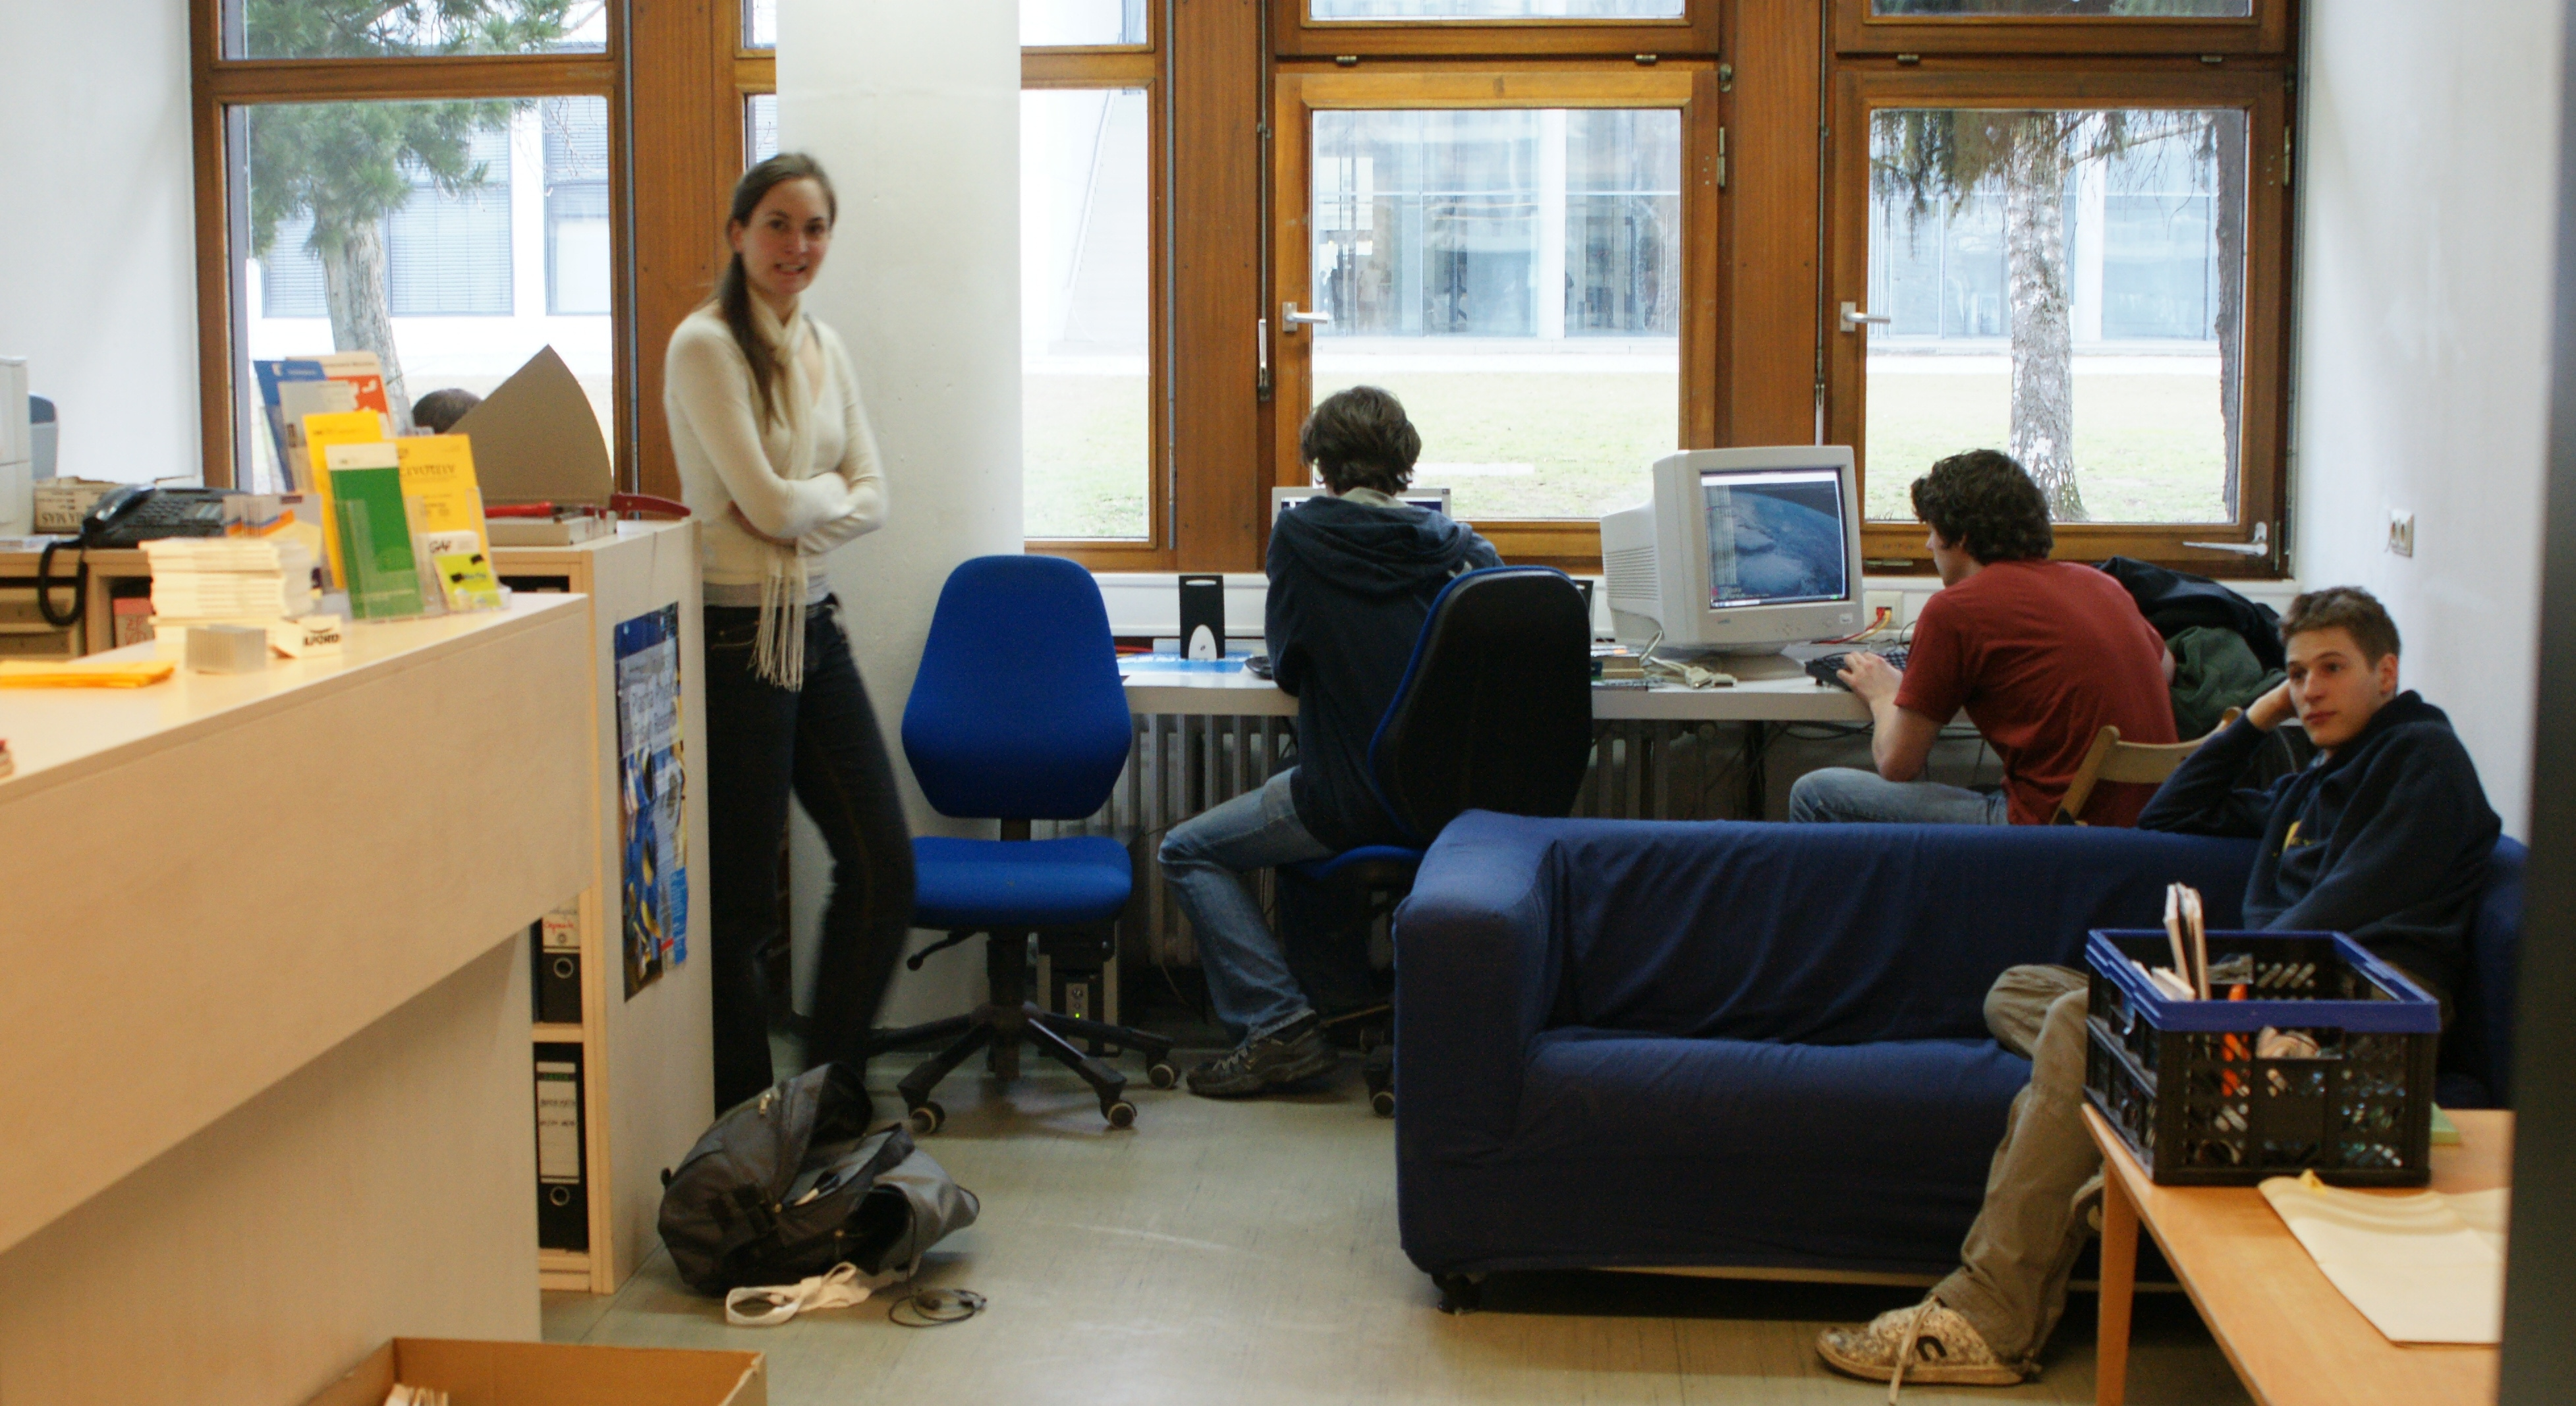
\includegraphics[width=0.8\textwidth]{aktive-fachschaft_print}}

	%\documentclass[12pt,a4paper]{scrbook}
%\usepackage[utf8]{inputenc}
%\usepackage{amsmath}
%\usepackage{amsfonts}
%\usepackage{amssymb}
%\usepackage{graphicx}
%\usepackage{csquotes}

%\begin{document}
	
\chapter{Computer und Internet}
Hier erfährst du, welche Möglichkeiten du hast, die CIP-Pools (Computerräume) zu nutzen, die je nach Fach verschieden notwendig, hilfreich und ausgestattet sind, wie du Zugang zum Uni-WLAN erhältst 
und welche anderen nützlichen Dinge die Uni online anbietet.

%TODO? Druckerkontingent (I/MI): gemeinsames Kontingent für Farbe und S/W (Eine Farbseite kostet 3 Seitenwerte)
%TODO Rechner in Theresienstraße (I/MI) muss erst “freigeschalten” werden (remote-enabler auf https://tools.rz.ifi.lmu.de/cipconf/index.rb?op=remote)
% evtl. Infos wo/wie man sein verbleibendes Kontingent anschauen kann
%TODO: Cip-Pool Theresienstraße(I/MI): Um sich an den Rechnern anzumelden, erst Strg-alt-Backspace drücken, um
% Anmeldemaske für Informatik auszuwählen
\section{CIP-Pools}
In CIP-Pools\footnote{Computer-Investitions-Programm} findest du Rechnerarbeitsplätze und Drucker, teilweise auch Scanner. Das Druckerkontingent beträgt für Mathematika, Physika und Statistika 500 Seiten pro Semester. Informatika haben 600 Seiten pro Semester zur freien Verfügung. Einige CIP-Pools haben auch Farbdrucker, deren Kontingent ist kleiner (für Informatiker kostet eine Farbseite so viel wie drei schwarz-weiß Seiten).

\begin{tabularx}{\linewidth}{lX}
\textbf{Mathematik, Wirtschaftsmathematik} %\subjectList{\subjectM\subjectW}
& Theresienstraße 37--41, BU135 und BU136, Wendeltreppe nach unten\\
\textbf{Physik, Meteorologie} %\subjectList{\subjectP}
& Schellingstraße 4 Erdgeschoss, H037 und H022\\
\textbf{Medieninformatik, Informatik}  %\subjectList{\subjectMI\subjectI}
& Oettingenstraße 67, BU102, LU112, LU114 und LU117 (Keller und Barracken)\\
\textbf{Medieninformatik zusätzlich} %\subjectList{\subjectMI}
& Amalienstraße 17, EG\\
\textbf{Für alle}    %\subjectList{\subjectP\subjectI\subjectMI\subjectM\subjectW}
& Theresienstraße 37--41, 1. Stock B115 \newline
%\footnotesize{$^*$Physik: arbeiten, nicht drucken \newline $\phantom{^*}$Informatik: drucken, nicht arbeiten}
\end{tabularx}

\begin{center}
	{
\includegraphics[width=0.6\textwidth]{comic_virus}}
\end{center}

\section{Online-Dienste der LMU}
\label{sec:online}
\subsection*{Campus LMU}
\begin{itemize}
	\item Aktivierung der Campus-Kennung
	\item Zugang zum E-Mail-Account
	\item Zugang zum Benutzerkonto (An-/Abmeldung von Newslettern der LMU)
	\item Zugang zum LSF (Vorlesungsverzeichnis)
\end{itemize}
\begin{urlList}
	\urlItem{http://www.portal.lmu.de}
\end{urlList}

\begin{center}
	{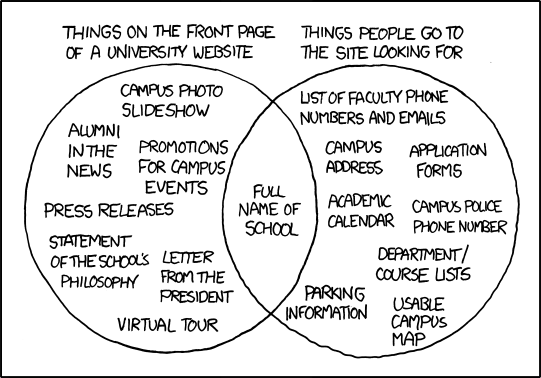
\includegraphics[width=0.6\textwidth]{comic_university}}
\end{center}

\subsection*{Online-Selbstbedienungsfunktionen}
\begin{itemize}
	\item Bescheinigungen für Immatrikulation, Studienverlauf, gezahlte Beiträge. Diese sind online noch vor dem Versand der offiziellen Bestätigungen verfügbar (nützlich für Arbeitsverträge).
	\item Änderung von Adressdaten und Telefonnummern
	\item Formular zur Prüfungsanmeldung
\end{itemize}
\begin{urlList}
	\urlItem{http://www.lmu.de/studium/studium_aktuell/neuigkeiten/studkanz/system.html}
\end{urlList}

\subsection*{Vorlesungsverzeichnis (Lehre Studium Forschung -- LSF)}
\begin{itemize}
	\item Übersicht über (fast) alle Veranstaltungen der LMU
	\item Stundenplan-Tool (etwas merkwürdig zu bedienen)
	\item Anmeldung zu Kursen und Klausuren (BWL, VWL)
	\item Notenauszug, in der Physik nicht immer aktuell
\end{itemize}
\begin{urlList}
	\urlItem{http://www.lsf.lmu.de}
\end{urlList}


\subsection*{E-Medien}
Viele E-Books, Paper, und wissenschaftliche Journale bekannter Wissenschaftsverlage stehen LMU Mitgliedern kostenlos zur Verfügung.
Besucht man die Webseiten der entsprechenden Publikationen, fordern die Verlage einen zum Kauf auf.
Besucht man die Webseite jedoch über den E-Medien-Login der Universitätsbibliothek \ref{emedien} stehen einem die Werke kostenlos zum Download bereit.
\begin{urlList}
	\urlItem{http://emedien.ub.uni-muenchen.de/}[emedien]
\end{urlList}

\subsection*{Microsoft DreamSpark \subjectList{\subjectI{}\subjectMI{}\subjectP{}}}
Studika der Physik und Informatik (auch im Nebenfach) bekommen über
Microsoft DreamSpark (früher MSDNAA) viele Microsoftproduktlizenzen
gratis, darunter Windows, Visual Studio und viele
Microsoft Office-Komponenten, jedoch \textbf{nicht} Word, Excel und PowerPoint.

\begin{urlList}
	\urlItem{http://tools.rz.ifi.lmu.de/cipconf/index.rb?op=msdnaa}
	\urlItem{https://msdnaa.physik.uni-muenchen.de/}
\end{urlList}

\subsection*{UniWorX\subjectList{\subjectI{}\subjectMI{}}}
\begin{itemize}
	\item Anmeldung zu Kursen und Klausuren
	\item Einsicht deiner Noten und Statistiken zu deinen Klausuren
	\item Abgabe von Übungsblättern
	\item Mit Campus- oder CIP-Kennung nutzbar
\end{itemize}
\begin{urlList}
	\urlItem{http://www.uniworx.ifi.lmu.de}
\end{urlList}

\subsection*{Prüfungsverwaltungs- und Informationssystem (PVI)\subjectList{\subjectI{}\subjectMI{}}}
\begin{itemize}
	\item Notenauszug, verbuchte Prüfungen
\end{itemize}
\begin{urlList}
	\urlItem{http://pvineu.ifi.lmu.de}
\end{urlList}




\section{E-Mail}
Damit du nicht unterfordert wirst, besitzt du direkt von Anfang an mindestens zwei verschiedene E-Mail-Adressen. Bei beiden E-Mail-Adressen ist es möglich und auch wärmstens empfohlen eine Weiterleitung einzurichten.

Die Campus-Adresse besitzt jedes Studikon der LMU, während die CIP-Adresse für die Nutzer der CIP-Pools ist.


\subsection*{Mathematik und Wirtschaftsmathematik\subjectList{\subjectM\subjectW}}
\begin{itemize}
	\item[]<seltsameKombination>@math.lmu.de
\end{itemize}
Deinen Account kannst du bei Herrn Spann (Theresienstraße 37--41, B124) beantragen. Die Weiterleitung erfolgt über das Shell-Kommando \verb|echo "neue Adresse" >~/.forward|. 

\subsection*{Informatik und Medieninformatik \subjectList{\subjectI\subjectMI}}
\begin{itemize}
	\item[]<accountname>@cip.ifi.lmu.de
\end{itemize}
Sollte unbedingt abgerufen oder weitergeleitet werden, da hierüber der Großteil des Informatik-Mailverkehrs abläuft. Das Passwort wird während der Anmeldung vergeben, die Kennung kannst du während der O"~Phase, in den ersten zwei Wochen des Semesters zu Blockterminen oder nach dem 15.Oktober zu den Sprechstunden der RBG\footnote{Rechnerbetriebsgruppe} 
(Mo--Do, 14--17 Uhr) jeweils in der Oettingenstraße 67, in LU113. beantragen-

\begin{urlList}
		\urlItem{https://webmail.ifi.lmu.de}
		\urlItem{http://www.rz.ifi.lmu.de/Dienste/Mailsystem.html}
\end{urlList}

\subsection*{Physik und Meteorologie\subjectList{\subjectP}}
\begin{itemize}
	\item[]<vorname.nachname>@physik.uni-muenchen.de
\end{itemize}
An diese Adresse werden Ankündigungen des Prüfungsamtes und Physik-Newsletter gesendet.
Das Passwort ist dasselbe wie für die Campus-Adresse.

\begin{urlList}
	\urlItem{http://webmail.physik.uni-muenchen.de}
	\urlItem{http://www.it.physik.uni-muenchen.de/dienste/kommunikation/e-mail}
\end{urlList}

\subsection*{Für alle Studika der LMU}
\begin{itemize}
	\item[]<vorname.nachname>@campus.lmu.de (bzw. was ihr angegeben habt)
\end{itemize}
Zum Weiterleiten einfach unter \ref{webmail} links unten auf Weiterleitung klicken und eine andere E-Mail-Adresse angeben.

\begin{urlList}
	\urlItem{https://mailbox.portal.uni-muenchen.de}[webmail]
\end{urlList}

\section{IRC}
IRC ist ein steinaltes, minimalistisches und nicht totzukriegendes
Chatprotokoll für Dinge, die nicht ganz eine E-Mail wert sind. Während die Uni
es nicht offiziell nutzt, ist es beliebt unter Studenten, speziell unter
Informatikern und uns Fachschaftlern. Manch einer zieht es sogar Facebook vor!

Das IRC ist aufgeteilt in Kanäle, die auf Netzwerken leben. Um dich zu einem
Netzwerk zu verbinden, brauchst du meist einen Client, aber viele Netzwerke
bieten für Anfänger auch Webchats an. Uns findest du im Kanal \#gaf auf dem
Netzwerk freenode.

\begin{urlList}
	\urlItem{http://www.irchelp.org/irchelp/clients/}
	\urlItem{https://webchat.freenode.net/}
\end{urlList}



\section{Internet / WLAN}
Um mit deinem Laptop in der Uni ins Internet zu gehen, brauchst du
deine Campus-Kennung. Damit lassen sich die WLAN-Services des
Leibniz-Rechen\-zentrums (LRZ) nutzen.

\subsection*{Eduroam}
Wir empfehlen dir, das WLAN mit dem Namen (SSID) \emph{eduroam}, auf deinen Geräten einzurichten. Mit diesem einmal eingerichteten Eduroam kannst du weltweit an vielen Universitäten und Forschungsinstituten automatisch das dortige WLAN nutzen. Unter \ref{eduroam} findest du ausführliche Anleitungen für die meisten Betriebssysteme und Smart\-phones 
(die benötigte LRZ-Kennung findest du in deinem Campus-Account unter `Benutzerkonto' $\rightarrow$ `E-Mail-Einstellungen').

%TODO noch ein Hinweis auf das weniger gefüllte eduroam-a?
Falls du nun in der Uni sitzt und dich fragst, wie du ohne Internet
die Anleitung durchlesen oder deine LRZ-Kennung herausfinden sollst, 
findest du die Antwort im Abschnitt LRZ.
\begin{urlList}
	\urlItem{http://www.lrz.de/services/netz/mobil/eduroam}[eduroam]
\end{urlList}

\subsection*{LRZ}
Außer Eduroam gibt es noch die Möglichkeit, das Netz mit der SSID
\emph{lrz} zu verwenden. \emph{lrz} ist zunächst ein unverschlüsseltes
Netzwerk, das nur den Zugriff auf die Website des
Leibniz-Rechen\-zentrums gestattet. Hier kannst du dir entweder die 
Anleitung für \mbox{\emph{eduroam}} durchlesen, oder die
vorkonfigurierte Clientsoftware AnyConnect herunterladen, welche dich
durch Anmeldung mit deiner Campuskennung in ein VPN (Virtual Private
Network) des LRZ einbucht. Aus Netzwerksicht verhält sich dein Rechner
dann wie alle anderen Rechner im MWN (Münchner Wissenschaftsnetz). So
kannst du nicht nur normal surfen, sondern auch von außen auf das
MWN zugreifen um zum Beispiel bestimmte Artikel aus der Bibliothek zu lesen.

Die Clientsoftware ist übrigens außerhalb der Uni praktisch, um deine
HTTP"=Verbindungen zu verschlüsseln, etwa wenn du dich in einem
ungeschützen WLAN befindest.

%\end{document}

	
\section{Vorlesungszeit}

\subsection{Der Stundenplan}

Wenn man ein neues Semester beginnt, egal ob das erste oder ein späteres, ist das Wichtigste, einen Stundenplan zu haben.


Das Vorlesungsverzeichnis findest du unter: \url{www.lsf.lmu.de}

Auf den Fakultätsseiten gibt es zum Teil noch eine kommentierte
Version. In der Aktualität wechseln sich die beiden Seiten ab, meist
ist die kommentierte Version jedoch vollständiger.

Die Erstellung über das lsf ist sehr kompliziert und weniger
empfehlenswert.  Wichtig ist, dsas du explizit auf ``Plan Speichern''
klickst!  Papier vergisst nichts.

\begin{itemize}
	\item Sortiere nach verbindlichen und empfohlenen Veranstaltungen.
	\item Plane erst obligatorische Veranstaltungen (Studienplan).
	\item Beachte Lehrveranstaltungszyklen (Was baut aufeinander auf?)
	\item Beachte, ob eine Lehrveranstaltung nicht in jedem
          Semester angeboten (z.b. nur jährlich) wird und ob
          Vorlesungen und Seminare oder Übungen im Zusammenhang
          stehen.
	\item Plane Lehrveranstaltungen in einem Umfang von höchstens 20 Semesterwochenstunden, denn Übungen, Tutorien, Selbststudienzeiten sowie Vor- und Nachbereitungen sind in jedem Fall notwendig.
	\item Beachte Wege und Fahrzeiten zwischen den Vorlesungen.
	\item Überprüfe den Stundenplan nach der ersten Vorlesungswoche in Bezug auf Mach- und Brauchbarkeit deines Plans.
	\item Erstelle darüber hinaus einen Semesterplan, in dem alle Termine, Fristen, Aktivitäten vermerkt sind, wie Rückmeldefristen, Klausuren, Referate oder Vorbereitungszeiten für Prüfungen.
	\item Schaue über den Tellerrand hinaus und tief in den Teller hinein. Die LMU bietet eine Vielzahl von Studiengängen an. Suche dir ruhig auch einmal etwas heraus, was dich zwar interessiert, du aber nicht in dein Studium einbringen kannst (von Arabistik bis Zoologie\ldots).
	\item Berücksichtige auch zusätzliche Veranstaltungen, wie beispielsweise Sprachen lernen, Computerkurse, Sport o.ä.
\end{itemize}


\subsection{Zusatz-Angebote}
\begin{itemize}
	\item Fremdsprachen: \url{www.sprachenzentrum.lmu.de}
	\item Ringvorlesung: \url{www.lmu.de/ringvorlesung}
	\item Studium Generale: \newline \url{www.lmu.de/studium/studienangebot/lehrangebote/studium_generale}
	\item LMU PLUS Seminare: \url{www.frauenbeauftragte.lmu.de/plus/plus_veranstaltungen}
	\item Soft Skills, Bewerbungstraining: \url{s-a.uni-muenchen.de} und \url{www.jobline.lmu.de}
	\item Soft Skills an der TUM: \newline \url{www.cvl-a.de/index.php?option=com_content&view=article&id=24}
\end{itemize}


\clearpage


\subsection{Zentraler Hochschulsport (ZHS)}
Für den körperlichen Ausgleich zum Studium kann man in kostspielige Fitnesscenter gehen oder aber eine der vielen interessanten Sportarten, wie z.B. Fechten, Segeln oder Bergsteigen ausprobieren, die vom ZHS zu einem relativ günstigen Preis (ab 7,50~€ pro Semester) angeboten werden. Der Großteil des Angebots findet auf dem Olympiagelände statt und ist -- abgesehen vom Fahrrad -- am besten mit der U3 (Haltestelle Olympiazentrum) und einem kurzen Fußmarsch durchs Olympische Dorf zu erreichen.

Das komplette Sportangebot könnt ihr der Homepage (\url{zhs-muenchen.de}) und dem Hochschulsportheft entnehmen, das zu Semesterbeginn unter anderem im Gumbel ausliegt.

Meistens ist eine Onlineanmeldung verpflichtend, damit du an den
Kursen teilnehmen darfst. Bringe deine Anmeldebestätigung ausgedruckt
mit. Für die Teilnahme brauchst du einen ZHS-Ausweis der
entsprechenden Kategorie mit gültigen Sportmarken, welche online
gebucht werden müssen. Danach musst du dir mit ausgedruckter
Buchungsbestätigung, Studentenausweis, Lichtbildausweis und Passfoto
in der ZHS einen Ausweis erstellen lassen und die entsprechenden
Marken besorgen. In der ersten Woche des Semesters ist das auch in der
Innenstadt (Schellingstr. 3) möglich.



\subsection{Essen}

Die verschiedenen Mensen des Studentenwerks mit Speiseplänen findet ihr unter\\ \url{studentenwerk-muenchen.de/mensa}. Zum Bezahlen braucht man eine Mensakarte, die man dort erwerben und aufladen kann.

In manchen Universitätsgebäuden ist darüber hinaus eine Cafeteria zu finden mit ähnlich preiswerten Essensangebot (Hauptgebäude (HGB) Nordhof, Schellingstr. 1. Stock, Oettingenstr. Keller, Giselastr. Mensagebäude).

Auch wenn du dir selbst ein Bild machen solltest, hier vorab ein Testbericht der Süddeutschen zu den verschiedenen Mensen:
sueddeutsche.de/muenchen/uni-mensen-im-test-\newline voll-auf-die-geschmacksnerven-1.32268

Wenn dir das Essen in den Mensen auf Dauer zu langweilig wird und du trotzdem nicht viel Geld ausgeben willst, hier ein paar Geheimtipps:

\begin{itemize}
	\item \textbf{Finanz- bzw. Landwirtschaftsministerium} (Odeonsplatz 4 bzw. Ludwigstr. 2): Ausschließlich für Mitarbeitern und Studenten. Darum musst du auch einen gültigen (Münchener) Studentenausweis und manchmal zusätzlich deinen Personalausweis vorzeigen. Es gibt täglich wechselnde Gerichte zu Preisen von 3,90~€ bis 6,00~€, jeden Mittwoch ist der allseits beliebte “Schnitzeltag” (4,10~€ mit Salat und Beilage).

	\item \textbf{HFF-Mensa (Hochschule für Film und Fernsehen)}
          (Bernd-Eichinger-Platz 1, gegenüber der TUM-Mensa): Etwas
          teurer als unsere Mensa, dafür aber besser.
\end{itemize}

	\chapter{Vorlesungsfreie Zeit}

\ldots heißt deshalb nicht Ferien, sondern vorlesungsfreie Zeit, weil man hier
endlich die Zeit hat in Ruhe zu lernen, Klausuren zu schreiben und
Blockseminare sowie Praktika zu besuchen. Die Uni kalkuliert die
Arbeitsbelastung so, dass man übers Jahr gerechnet etwa 6 Wochen Ferien hat, wie
ein normaler Arbeitnehmer auch.

\section{Klausuren und Protokolle}
Wir von der GAF sammeln Altklausuren und mündliche Prüfungsprotokolle. Das
meiste davon findest du in unserer Online-Sammlung \ref{klausuren}.
Benutzername und Passwort kannst du bei uns in der GAF erfragen oder dir per
E-Mail \ref{daten} zuschicken lassen.  Es existieren auch noch einzelne
ungescannte Protokolle von mündlichen Prüfungen, die du zum Kopieren ausleihen
kannst, vor allem von Physikern, die relativ selten gefragt wurden. Im
Zweifelsfall schaue zuerst online nach, falls du dort nichts findest, kannst
du gerne in unseren Ordnern suchen.

Damit auch künftige Generationen davon profitieren, schickt bitte alles,
was ihr in die Hände bekommt, (sofern noch nicht vorhanden) an uns.
Wenn du in einer Klausur sitzt, in der die Offiziellen mit Strafen
drohen, wenn jemand die Klausuren mitnimmt/abschreibt, erstellt
direkt im Anschluss ein Gedächtnisprotokoll.

Die Nächsten werden es euch danken!

\begin{urlList}
	\httpsItem{gaf.fs.lmu.de/klausuren}{klausuren}
	\httpsItem{gaf.fs.lmu.de/zugangsdaten/zugangsdaten.html}{daten}
\end{urlList}


	\chapter{Bibliotheken}

\section{Bücher}

Bei Verständnisschwierigkeiten des Stoffes hilft es -- neben
Kommilitonen um Rat zu fragen -- Bücher zu lesen.  Die Bibliothek
hat einen großen Bestand an Büchern, welche teilweise auch ausleihbar
sind. In der Regel sind die von den Professoren empfohlenen Bücher
mehrfach vorhanden, allerdings oft auch schnell vergriffen. Falls ein
von dir benötigtes Buch nicht vorhanden sein sollte:
Anschaffungswünsche werden innerhalb von etwa einem Monat erfüllt.

%TODO Hinweis auf EBooks zum Beispiel mit Verweis auf pcundinternet.tex

\section{Recherche im OPAC}
	\begin{urlList}
		\urlItem{http://opacplus.ub.uni-muenchen.de}
		\urlItem{http://www.ub.lmu.de}
	\end{urlList}

\section{Verhalten in der Bibliothek}
Verboten sind je nach Bibliothek: Rauchen, Essen, Getränke (außer Wasser in Plastikflaschen), Mäntel, Jacken, Taschen, Handyklingeln, Unterhalten.\\
Die Verbote variieren je nach Einrichtung relativ stark. Bitte informiere dich vorher online darüber.
Die Bibliotheken werden auch gerne einfach als ruhiger Ort zum Lernen genutzt.

\textbf{Bitte verhalte dich leise!
Deine lernenden Kommillitonen werden es dir danken.}

\section{Ausleihe}

Bücher in der Zentralen Lehrbuchsammlung (ehemals
Studentenbibliothek) und anderen Fachbibliotheken sind fast alle
ausleihbar. Bei Präsenzbibliotheken ist die Ausleihe nur über das
Wochenende möglich.

Beachte die Ausleihfristen (Mahngebühren variieren je nach Bibliothek!). 
Verlängerungen sind unter \ref{verlängerung}
möglich, vorausgesetzt, du hast noch keine ausstehenden Mahngebühren.

Gebühren kannst du an den Automaten in der Theresienstraße sowie
im Hauptgebäude begleichen.

\begin{urlList}
	\urlItem{http://opacplus.ub.uni-muenchen.de}[verlängerung]
\end{urlList}

\section{Die wichtigsten Bibliotheken für dich}

\subsection*{Fachbibliothek für Mathematik, Physik und Meteorologie\subjectList{\subjectM\subjectW\subjectP}}
Theresienstr. 37 (1. Stock)\\
Öffnungszeiten: Mo -- Fr 8:00 -- 22:00~Uhr, Sa 9:00 -- 18:00~Uhr\\
Buchscanner, Kopierer/Scanner mit Kartenzahlung, Basisbibliothek aller
Studenten der Fakultäten 16/17, Diskussionsräume für Gruppenarbeit.
Zwei große Lese"~ und Arbeitssäale.

\subsection*{Fachbibliothek Englischer Garten\subjectList{\subjectI\subjectMI}}
Oettingenstr. 67 (Haupteingang, Erdgeschoss)\\
Öffnungszeiten: Mo -- Fr 8:00 -- 22:00~Uhr und Sa 9:00 -- 18:00~Uhr\\
Präsenzbibliothek Informatik, Münz- und Kartenkopierer, Ausleihe von max. fünf Büchern, nur für Informatik-Studenten und nur über das Wochenende (Fr, 11:00 -- Mo, 12:00~Uhr).

\subsection*{Zentralbibliothek der LMU}
Geschwister-Scholl-Platz 1 (Hauptgebäude Südtrakt)\\
Öffnungszeiten: Mo -- Fr 9:00 -- 22:00~Uhr, Fr 9:00 -- 17:00~Uhr\\
Serviceschalter: Mo -- Fr 9:00 -- 20:00~Uhr\\
Anlaufstelle bei verlorener Bib-Karte und Abholung von Büchern aus dem Zentralbestand.

\subsection*{Bibliothek der TUM in der Innenstadt}
Arcisstr. 21d\\
Öffnungszeiten: Mo -- Fr 8:00 -- 24:00~Uhr, Sa, So und Feiertage 10:00 -- 22:00~Uhr\\
Für alle Studenten frei zum Lernen, einen TUM-Bibliotheksausweis erhältst du gegen Vorlage des Studienausweises an der Information.

\begin{urlList}
	\urlItem{http://www.ub.tum.de}
\end{urlList}

\subsection*{Bayerische Staatsbibliothek (Stabi)}
Ludwigstr. 16\\
Öffnungszeiten Ortsleihe: Mo -- Fr 10:00 -- 19:00~Uhr\\
Öffnungszeiten Lesesaal: täglich (auch Sonntags!) 8:00 -- 24:00~Uhr\\
Gewaltiger Bestand (Noten, Zeitschriften, Antikes\ldots), Bücher
müssen online bestellt werden, Ausleihe mit deiner LMU-Bib-Karte. Wer
einen Arbeitsplatz ergattern möchte, sollte früh da sein; der
Ansturm an Lernwilligen ist immens.
Es herrschen jedoch auch relativ strenge Benutzungsbedingungen, so wird der Wachmann schonmal nervös, wenn man in größeren Gruppen dort aufschlägt.
Zum Trinken darf auch nur Wasser in durchsichtigen Flaschen mitgebracht werden.

\begin{urlList}
	\urlItem{http://bsb-muenchen.de}
\end{urlList}

\subsection*{Bibliothek des Deutschen Museums}
Auf der Museumsinsel\\
Öffnungszeiten: täglich (auch Sonntags!) 9:00 -- 17:00~Uhr\\
Große Auswahl an technischen und naturwissenschaftlichen Werken, Präsenzbibliothek, schönes Gebäude.

\begin{urlList}
	\urlItem{http://deutsches-museum.de/bibliothek}
\end{urlList}

\subsection*{Münchener Stadtbibliothek (Hauptstelle am Gasteig)}
Rosenheimer Str. 5\\
Öffnungszeiten: Mo -- Fr 10:00 -- 19:00~Uhr und Sa 11:00 -- 16:00~Uhr\\
Rückgabe täglich 7:00 -- 23:00~Uhr\\
Niederlassungen über die ganze Stadt verteilt, Ausleihe für Studenten 10~€ pro Jahr.

\begin{urlList}
	\urlItem{http://muenchner-stadtbibliothek.de}
\end{urlList}

	
\section{Café Gumbel}

Das Café Gumbel ist ein vor Jahrzehnten erstreikter Aufenthalts- und Lernraum mit Teeküche.  Das Gumbel wird von Studika betrieben.  Während der
Öffnungszeiten ist der Raum inklusive Küche mit Wasserkocher und Geschirr
jedem zugänglich.

Falls du gerne einen Poetry Slam, Spieleabend oder
eine andere Veranstaltung für dich und deine Kommilitonen organisieren
möchtet, frag einfach an.  Wir stellen euch gerne einen Beamer, Soundanlage,
Spielkarten (usw.) zur Verfügung.

Theresienstr., B030\\
Mo -- Fr: 8:00 -- 22:00~Uhr (meistens)\\
Kontakt: \url{gumbel@fs.lmu.de}

\skiptobottom
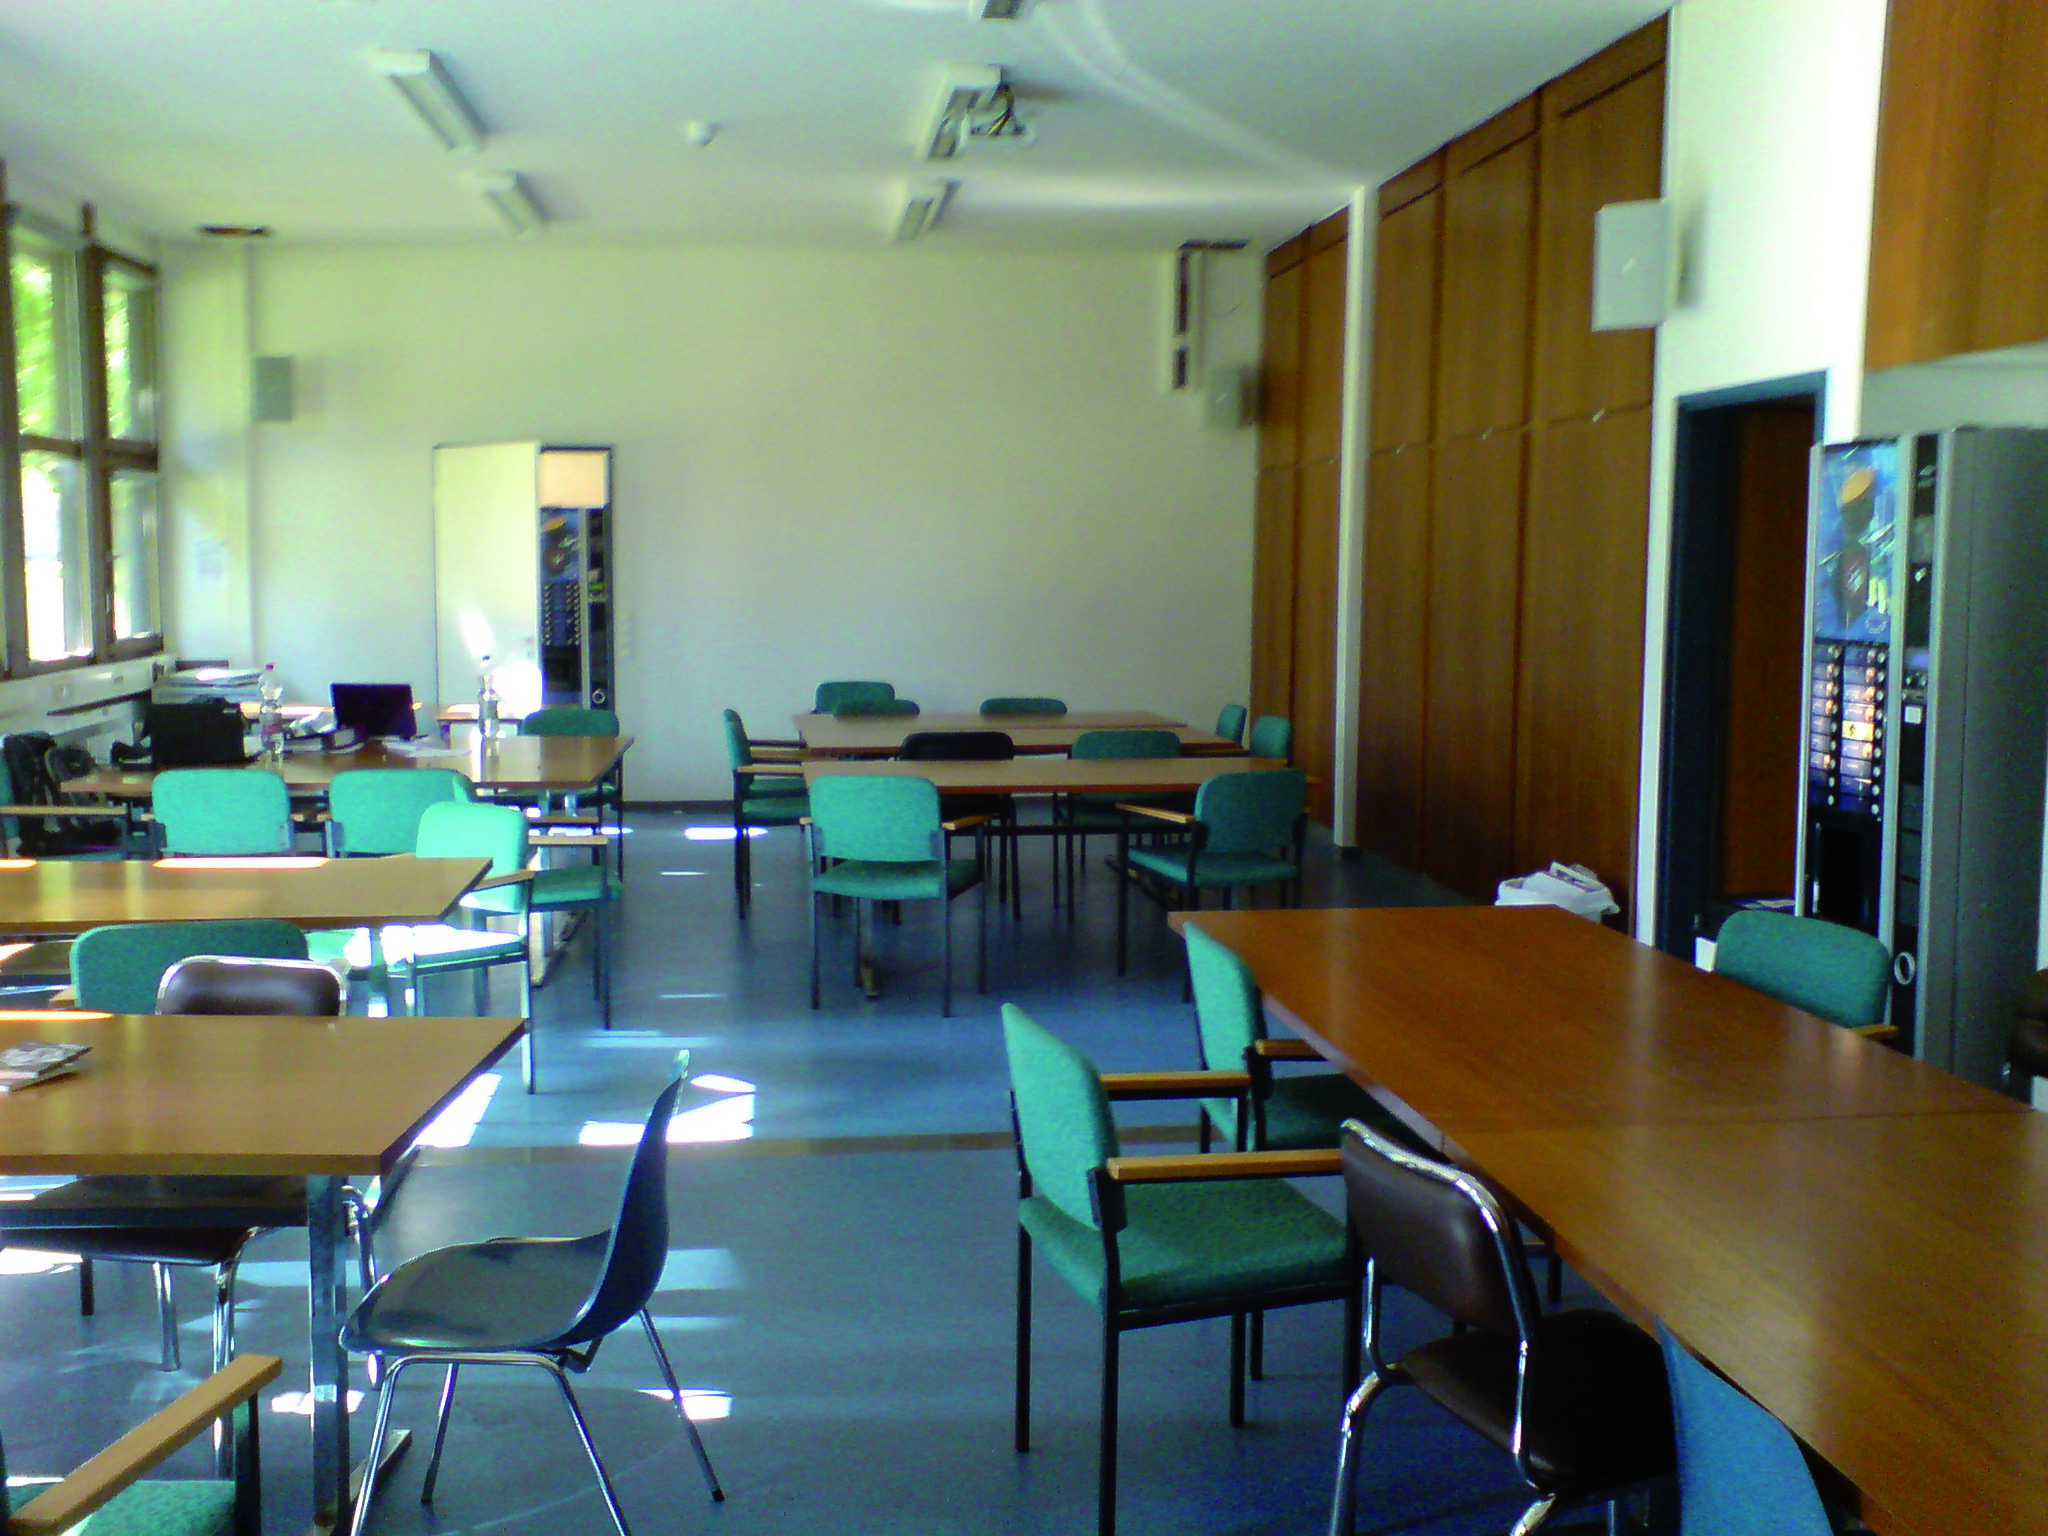
\includegraphics[width=\textwidth]{gumbel_raum_print}

	\chapter{Hilfe und Beratung}

\section{Erste Hilfe: GAF}

Wir kennen nicht immer die Lösung, wissen dafür aber meistens, wer sie
kennt. Wir haben gute Kontakte zu vielen Institutionen und Personen an
dieser Uni. Wenn du uns einfach mal besuchen willst, bist du herzlich
willkommen. (Kontakt siehe Kapitel \ref{gafKontakt}, S. \pageref{gafKontakt})


\section{Webforen und Kommilitonen}

In den Foren kannst du dich mit deinen Kommilitonen
(und teils auch mit Lehrpersonal) austauschen. Wenn du Fragen direkt zu den
Übungen oder der Vorlesung hast, kannst du dich auch einfach an die
Übungsleiter der jeweiligen Vorlesung wenden. Keine Sorge, die beißen nur
selten.

Wenn du im IRC (ein Chat-System) unterwegs bist, findest du unter \#gaf und \#informatik.lmu auf
freenode auch immer andere Studenten aus deinem Fach.

\begin{urlList}
	\urlItem{http://die-informatiker.net}
% 	\urlItem{http://die-physiker.org}
%	\urlItem{http://die-mathematiker.net}
\end{urlList}

\skiptobottom
\begin{center}
	{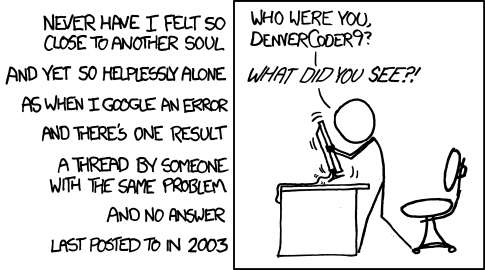
\includegraphics[height=3.5cm]{img/wisdom_of_the_ancients}}
\end{center}

%\begin{figure}[h]
%\centering
%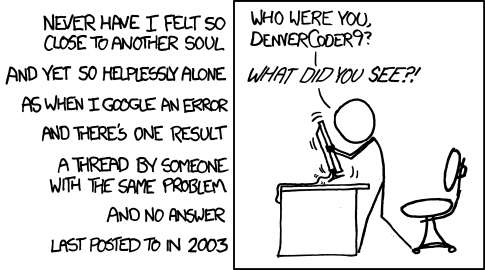
\includegraphics[height=3cm]{img/wisdom_of_the_ancients}
%\caption{}
%\label{fig:wisdom_of_the_ancients}
%\end{figure}


\newpage %% Das soll wieder raus

\section{Probleme mit Lehrveranstaltungen oder Lehrpersonal}

Die offizielle Ansprechperson hierbei ist der Studiendekan deiner
Fakultät. Er ist für die Qualität der Lehre verantwortlich. In jedem
Fall ist der sinnvollste Weg zu einer Lösung erst einmal das direkte
Gespräch mit dem Dozenten. Erst wenn ihr das Gefühl habt, ein Problem
lässt sich nicht anders lösen, bittet euren Studiendekan um
Hilfe. Oder fragt uns von der GAF.

\subsection*{Studiendekane Fakultät 16}
Prof. Werner Bley (Mathematik)\subjectList{\subjectM\subjectW}\\
Prof. Hans Jürgen Ohlbach (Informatik)\subjectList{\subjectI\subjectMI}\\
Prof. Thomas Augustin (Statistik)

\subsection*{Studiendekan Fakultät 17}
Prof. Dr. Jochen Weller \subjectList{\subjectP}

\section{Ansprechpartner nach Studiengängen}

Alle nachfolgenden Personen sind sehr umgängliche Menschen, mit denen
man bestens reden kann. Wie die meisten Professoren beißen sie nicht,
wenn man etwas zu beanstanden hat.

\subsection*{Mathematik (B.Sc., LA Gymnasium)\subjectList{\subjectM}}
PD Dr. Heribert Zenk (\mail{Heribert.Zenk@mathematik.uni-muenchen.de})\\
Theresienstraße 39, B333, Telefon: 089 / 2180 \emd{} 4460

PD Dr. Hartmut Weiß (\mail{hartmut.weiss@mathematik.uni-muenchen.de})\\
Theresienstraße 39, B317, Telefon: 089 / 2180 \emd{} 4680\\
Sprechstunde: Do, 15:00\emd{}16:00~Uhr

\subsection*{Wirtschaftsmathematik (B.Sc.)\subjectList{\subjectW}}
Prof. Dr. Gregor Svindland (\mail{studienberatung.wirtschaftsmathematik@math.lmu.de})\\
Theresienstraße 39, B231, Telefon: 809 / 2180 \emd{} 4628

\subsection*{Mathematik (LA Grund-, Haupt-, und Realschule)\subjectList{\subjectM}}
Dr. Erwin Schörner (\mail{schoerner@lmu.de})\\
Theresienstraße 39, B237, Telefon: 089 / 2180 \emd{} 4498

\subsection*{Mathematik (Fachdidaktik und Didaktik)\subjectList{\subjectM}}
Christoph Hammer (\mail{hammer@math.lmu.de})\\ %Akademischer Direktor?
Theresienstraße 39, B221, Telefon: 089 / 2180 \emd{} 4480

\subsection*{Informatik (B.Sc.)\subjectList{\subjectI}}
Dr. Reinhold Letz (\mail{reinhold.letz@lmu.de})\\
Oettingenstraße 67, E001, Telefon: 089 / 2180 \emd{} 9693\\
Sprechstunde: Di \& Mi 13:00\emd{}14:00~Uhr und nach Vereinbarung

\subsection*{Informatik (LA)\subjectList{\subjectI}}
Prof. Martin Hofmann, Ph.D. (\mail{lehramt@ifi.lmu.de})\\
Oettingenstraße 67, L107, Telefon: 089 / 2180 \emd{} 9341

\subsection*{Medieninformatik (B.Sc.)\subjectList{\subjectMI}}
Max Maurer / Simon Stusak (\mail{studentenbetreuer@medien.ifi.lmu.de})\\
Amalienstraße 17, 505, Telefon: 089 / 2180 \emd{} 4654

\subsection*{Physik (B.Sc.)\subjectList{\subjectP}}
Michael Rebhan (\mail{Michael.Rebhan@physik.uni-muenchen.de})\\
Schellingstraße 4, H417, Telefon: 089 / 2180 \emd{} 5033

\subsection*{Physik plus Meteorologie (B.Sc.)\subjectList{\subjectP}}
Dipl. Met. Heinz Lösslein (\mail{loesslein@lmu.de})\\
Theresienstraße 37, A208, Telefon: 089 / 2180 \emd{} 4217

\subsection*{Physik (LA)\subjectList{\subjectP}}
Prof. Dr. Raimund Girwidz (\mail{girwidz@physik.uni-muenchen.de})\\
Theresienstraße 37, A012, Telefon: 089 / 2180 \emd{} 2020


\section{Prüfungsamt}
Die Prüfungsämter sind für alle Prüfungsangelegenheiten zuständig,
also unter anderem für deine Noten, deine Praktika, deine Notenübersichten und
Abschlusszeugnisse. Sie sind bei der Fakultät zu finden, zu der
dein Studienfach gehört. Eine Zuordnung der Prüfungsämter zu den
einzelnen Studiengängen/-fächern findest du auf der Übersichtsseite
Studiengänge A--Z am unteren Ende der jeweiligen
Studiengangsinformationen.

\begin{urlList}
	\urlItem{http://www.lmu.de/pruefungsaemter}
\end{urlList}


\section{Studentenkanzlei}

Die Studentenkanzlei muss wegen gewissen formalen Belangen
gelegentlich besucht werden. Der Besuch dieses kafkaesken Molochs ist
oft mit großen Wartezeiten und Unbill verbunden. Es hilft, hartnäckig
zu bleiben und notfalls mehrfach zu kommen, bis du den richtigen
Sachbearbeiter triffst. Nicht umgehen lässt sich ein Besuch bei:

\begin{itemize}
\item Beantragen von Beurlaubungen (Krankheit, Ausland, Kinder, \ldots)
\item Fragen zur Studienplatzvergabe/\,Immatrikulation (Anerkennung von Hochschulzugangsberechtigungen, nachträgliches Einschreiben, Verlust der Immatrikulationsbescheinigung)
\item Studienfachwechsel, zusätzliche Einschreibung für ein Doppelstudium
\item Bescheinigungen für die Krankenkasse und Rente, Quittungen für Studienbeiträge
\end{itemize}

Die Studentenkanzlei ist in den Räumen E011 und E114 im Hautgebäude zu finden und Montag bis Mittwoch, sowie am Freitag von 8:30 bis 11:30~Uhr geöffnet, am Donnerstag von 13:30 bis 15:00~Uhr.

\begin{urlList}
	\urlItem{http://www.lmu.de/studentenkanzlei}
\end{urlList}


\section{Studieren mit Kind}

Auch für Eltern ist Studieren nicht unmöglich. Die Uni bietet diverse Beratungs"~ und Betreuungsmöglichkeiten.

\begin{urlList}
	\urlItem{http://studentenwerk-muenchen.de/studieren-mit-kind}
	\urlItem{http://www.lmu.de/studium/beratung/beratung_service/beratung_lmu/schwangere_kind}
\end{urlList}

%\section{Gleichstellungsbeauftragte}
%
%\begin{urlList}
%	\urlItem{www.gleichstellungsbeauftragte.lmu.de}
%\end{urlList}

\section{Die Frauenbeauftragten}
Weitere Anlaufstellen im Uni-Alltag vor allem bei Fragen und Problemen bezüglich Diskriminierungen und sexueller Belästigung im Wissenschaftsbetrieb sind die Frauenbeauftragten.
Das Aufgabengebiet der Frauenbeauftragten ist vielfältig und groß, darum hat zusätzlich zur Universitätsfrauenbeauftragten jede Fakultät eigene Frauenbeauftragte.

Alle Studierende können an den Weiterbildungsprogramm LMU-PLUS, welches durch das Büro der Frauenbeauftragten organisiert und aus Studienersatzmitteln finanziert wird, teilnehmen. Ausschließlich zur Förderung von Frauen ist das LMUMentoring und die Beratung zur finanziellen Förderung von Nachwuchswissenschaftlerinnen gedacht.

\begin{urlList}
	\urlItem{http://www.frauenbeauftragte.uni-muenchen.de/weiterbildung/plus/index.html}
	\urlItem{http://www.mathematik-informatik-statistik.uni-muenchen.de/fakultaet/beauftragte/index.html}
	\urlItem{http://www.physik.uni-muenchen.de/fakultaet/einrichtungen/frauenbauftragte/index.html}
\end{urlList}


\section{Studieren mit Behinderung}

Solltest du aufgrund einer Behinderung mehr Zeit, spezielle Hilfsmittel oder einen eigenen Raum für Klausuren benötigen, so kannst du beim Prüfungsamt einen Nachteilsausgleich beantragen.

\begin{urlList}
	\urlItem{http://studentenwerk-muenchen.de/studieren-mit-behinderung}
	\urlItem{http://www.lmu.de/barrierefrei}
\end{urlList}


\section{Student und Arbeitsmarkt}

Der Career Service der Universität bietet dir eine Stellen- und Praktikavermittlung, Kompetenztrainings, ein Mentoringprogramm, verschiedene Recruitung Events und einiges mehr. Einen Überblick verschaffst du dir am besten online oder du besuchst den Career Service in der Ludwigstraße 27 / I. Stock am Montag, Dienstag, Donnerstag und Freitag zwischen 10 und 12~Uhr.

\begin{urlList}
	\urlItem{http://www.s-a.lmu.de}
\end{urlList}


\section{Psychosoziale Beratung}

Wenn du das Gefühl hast, die Kontrolle zu verlieren oder nicht mehr mit
dem Studium und/oder den Menschen um dich herum zurecht kommst, wende dich an die kostenlose Psychosoziale Beratung des Studentenwerks.

\begin{urlList}
	\urlItem{http://www.studentenwerk-muenchen.de/beratungsnetzwerk/psychosoziale-und-psychotherapeutische-beratung/}
\end{urlList}


\section{Weitere Beratung des Studentenwerks}
Helene-Mayer-Ring 9 (U3 Olympiazentrum)

\begin{itemize}
	\item Allgemeine und Soziale Beratung
	\item Psychotherapeutische Beratungsstelle
	\item Studienkreditberatung
	\item Rechtsberatung
	\item Wohnungsberatung/\,Privatzimmervermittlung
	\item Beratungsstelle \enquote{Sexuelle Belästigung, Diskriminierung und Gewalt}
	\item Beratung für ausländische Studierende
\end{itemize}

\begin{urlList}
	\urlItem{http://studentenwerk-muenchen.de/beratungsnetzwerk}
\end{urlList}


\section{Nightline München}

Die Nightline München ist ein Zuhörtelefon von Studika für Studika,
das abends und nachts zu erreichen ist. Am Telefon sitzen ehrenamtlich
tätige Studika, die dir mit einem offenen Ohr beistehen.

\begin{urlList}
	\urlItem{http://www.nightline.mhn.de/}
\end{urlList}


\section{Kirchliche Beratung}
Die christlichen Hochschulgemeinden bieten neben ihrem konfessionellen Angebot auch überkonfessionelle und psychologische Beratung und Aktivitäten, wie Ausflüge, Workshops und Spieleabende.

\begin{urlList}
	\urlItem{http://www.khg.lmu.de}
	\urlItem{http://www.esg.lmu.de}
\end{urlList}

	\chapter{Ausland und Praktika}

Auslandssemester oder -praktika machen sich immer gut im Lebenslauf
und sind nebenbei bleibende Erinnerungen, von denen viele von uns mehr
profitiert haben als von der ein oder anderen Vorlesung. Und falls du
dich für ein Thema besonders interessierst, bieten auch viele
Hochschulen im Ausland die Möglichkeit, eine Abschlussarbeit bei ihnen
zu verfassen bzw. verfassen zu lassen.

Hierbei wirst du uni-intern vom \emph{Referat Internationale Angelegenheiten} und dem Career Center \emph{Student und Arbeitsmarkt} unterstützt, aber auch von Hochschulgruppen wie AISEC oder IAESTE (vom DAAD gefördert).

\section{Auslandsstudium}

Die LMU verfügt über eine Reihe von Partnerhochschulen in aller
Welt. Der Austausch ist hier einfacher (Formalien, Anerkennung von
ECTS). Für die
Partnerhochschulen kann man sich nur ein Mal im Jahr bewerben, also am
besten frühzeitig über Fristen informieren und bewerben.
Ein Jahr vor der Abreise ist manchmal schon zu spät, um sich bei
allen Organisationen (insb. DAAD) zu bewerben.
Es ist aber auch möglich, sich selbst einen Austausch an einer anderen
Hochschule zu organisieren.

Falls du im Ausland erworbene ECTS an der LMU anerkennen lassen
möchtest, solltest du dies im Vorfeld mit dem Studiengangskoordinator
abklären.

Austauschabkommen und -verträge, sowie Erfahrungsberichte findest du unter \ref{ausland}.

\begin{urlList}
	\httpsItem{www.moveon.verwaltung.uni-muenchen.de/move/moveonline/exchanges/search.php?_language=de}{ausland}
\end{urlList}

\section{Praktika im In- und Ausland}

Neben Jobbörsen gibt es auch Datenbanken wie die des DAAD mit
Praktikums"=Erfahrungsberichten. So kann man sich im Vorfeld schon
einen groben Überblick über das jeweilige Praktikum machen.

\begin{urlList}
	\httpItem{eu-community.daad.de/index.php?id=38}
\end{urlList}

\section{Finanzierung}

Dies ist nur eine Auswahl der Möglichkeiten. Für bestimmte Länder und
Vorhaben gibt es auch noch spezielle finanzielle Unterstützungen. Die
Vorlaufzeit beträgt 3 bis 18 Monate.

\begin{itemize}
\item Auslands-BAföG: staatliche finanzielle Förderung (nicht zurückzuzahlen) für ein Studium oder Praktikum im Ausland. Hierbei sind auch viele förderungsberechtigt, die kein reguläres BAföG erhalten, also auf jeden Fall bewerben!
\item ERASMUS: ein Stipendiumprogramm für ein 3- bis 12-monatiges Studium oder Praktikum im europäischen Ausland.
\item DAAD und PROSA LMU: Stipendien für Studium, Praktikum, Sprachkurse und Kurzprogramme im Ausland.
\end{itemize}

\subsection*{Referat Internationale Angelegenheiten}
HGB, G013, Zugang über G011

\begin{urlList}
	\httpItem{www.lmu.de/international/auslandsstudium}
\end{urlList}

\subsection*{Student und Arbeitsmarkt}

HGB, G206\\
Mo, Di, Do und Fr: 10:00--12:00~Uhr

\begin{urlList}
	\httpItem{www.s-a.lmu.de}
\end{urlList}


	
\chapter{Geld}

\section{Studentenwerksbeitrag}
Der Studentenwerksbeitrag setzt sich zusammen aus einem Grundbeitrag an das Studentenwerk (52,-€) und dem
Semesterticket-Sockelbeitrag (59,-€).
Diese 111,-€ müssen von allen Studika gezahlt werden, Ausnahme sind schwerbehinderte Studika, die Anspruch
auf unentgeltliche Beförderung haben.

\section{Jobben}
In München findest du eine Vielzahl an Nebenjobs: von Kellern oder Nachhilfe ($\geq$ 15~€/h) bis zu an der Uni selbst (ca. 8 -- 11~€/h). Deutlich höhere Stundenlöhne erhältst du, wenn du in einem der vielen IT-Unternehmen als Werkstudent arbeitest ($\geq$ 12~€/h).

Angebote findest du in Aushängen (Uni, Geschäfte) und Stadtmagazinen, aber auch in unseren Uni-Foren und unter den folgenden Adressen:
\begin{urlList}
	\httpItem{www.s-a.uni-muenchen.de/studierende/jobboerse/index.html}
	\httpItem{www.jobcafe.de}
	\httpItem{www.uni-muenchen.de/aktuelles/stellenangebote/stud_hilfskraft/index.html}
\end{urlList}

Beim Jobben solltest du den finanziellen Freibetrag der Krankenversicherung und gegebenenfalls beim BAFöG beachten, aber auch dass du unter den maximalen Wochenstunden bleibst (Krankenversicherung). Während dem Semester gelten dabei andere Grenzen als in den Semesterferien.

Dein Einkommen ist bis zu einer Grenze von ungefähr 8.000~€ (Freibetrag ohne Werbekosten usw.) steuerfrei.


\section{BAföG}
Im Studium kann man vom Staat finanzielle Unterstützung nach dem BundesAusbildungsförderungsGesetz erhalten. Grundsätzlich bekommen all diejenigen BAföG, die ihre Ausbildung nicht anderweitig finanzieren können (abhängig von deinem Einkommen und dem deiner Eltern / Fürsorgepflichtigen). Der Förderbetrag muss nach dem Studium zur Hälfte zurückgezahlt werden (zinsloses Darlehen), der Rest wird erlassen.

Einen ersten Eindruck von deiner Chancen auf BAföG bzw. die erwartbare
Höhe bekommst du mit dem BAföG-Rechner:
\begin{urlList}
	\httpItem{www.bafoeg-rechner.de/Rechner}
\end{urlList}

Bei einem Nein im Rechner kann es trotzdem sein, dass du BAföG
bekommst. Überlege, ob sich der Aufwand des Einreichens und
Nachreichens der Anträge für dich lohnt.

Die Bafög-Unterlagen erhältst du unter:
\begin{urlList}
	\httpItem{das-neue-bafoeg.de}
\end{urlList}
oder kannst sie online ausfüllen unter: 
\begin{urlList}
	\httpItem{bafoeg-bayern.de}
\end{urlList}

Für allgemeine Fragen kannst du dich an die allgemeine BAföG-Beratung des Studentenwerks wenden:

Helene-Mayer-Ring 9, Raum h4\\
Tel.: 089 357135-30\\
beratung-m@bafoegbayern.de\\
Mo, Di, Mi: 9:00--13:00~Uhr, 14:00--16:00~Uhr, Do: 9:00--13:00~Uhr, 14:00--17:00~Uhr, Fr: 9:00--13:00~Uhr

Konkrete Fragen besprichst du am Besten mit deinem Sachbearbeiter.

\section{Stipendien}
Stipendien haben meistens einen finanziellen und einen ideellen Anteil
(Seminare etc.). Für ein Stipendium ist neben passablen Noten vor
allem soziales Engagement wichtig.

\begin{urlList}
	\httpItem{www.lmu.de/deutschlandstipendium}
	\httpItem{www.lmu.de/studium/studienfinanzierung/stift}
\end{urlList}

Es gibt diverse weitere Stipendien, die nicht nur auf Noten achten.
Suchen lohnt sich!

	
\section{Ankommen in München}

\subsection{Ummeldung / Zweitwohnsitz}

Nach einem Umzug muss man sich in der neuen Stadt anmelden bzw. bei einem Stadtgebietwechsel ummelden. Entweder stattet man dazu dem KVR persönlich einen Besuch ab oder schickt das unterschriebene Formular per Post. Das Formular sowie nähere Infos zu den zuständigen Stellen finden sich im Internet im Dienstleistungsfinder auf den Seiten der Stadt München.

benötigte Unterlagen für die Ummeldung: %Als Liste, damit man alles auf einen Blick hat.
\begin{itemize}
	\item Personalausweis oder Reisepass
	\item bei mehreren Wohnungen: Das Beiblatt für mehrere Wohnungen
	\item bei der Anmeldung per Post: Ausgefülltes Formular und Kopie des Personalausweises.
\end{itemize}

Sollte man sich dafür entscheiden, München oder seine bisherige Wohnung als Zweitwohnsitz anzumelden, fallen extra Steuern an. Die Zweitwohnsitzsteuer liegt bei 9 \% der jährlichen Nettokaltmiete. Mit einem Nachweis über positive Einkünfte unter 25.000~€ ist eine Befreiung dieser Steuer möglich.

% Makros verwenden und ans ende!
\begin{urlList}
	\item \url{muenchen.de/dienstleistungsfinder/muenchen/1063475/}
\end{urlList}

\subsection{Mülltrennung}

Für die Restmüll- und Altpapiertrennung stehen in jedem Wohnblock eigene Tonnen zur Verfügung. Teilweise finden sich dort auch extra Biotonnen.
Die Container für Plastik, Dosen und Altglas sind über die Stadt verteilt und auch selten weit entfernt.
Sperrmüll, Elektroschrott und ähnliches sollte man am besten zu den Wertstoffhöfen bringen. Man sollte sich davor nach den Öffnungszeiten erkundigen. Im Gegensatz zu manch anderen Städten sind diese in München kostenlos.

% Makros verwenden!
\begin{urlList}
	\item \url{awm-muenchen.de}
\end{urlList}

%\subsection{Wohnung}
%\begin{itemize}
%	\item Die beliebtesten Portale für WGs: \url{wg-gesucht.de} und \url{studenten-wg.de} (Wenn ihr euch bewerbt, schreibt mehr als euren Namen und Telefonnummer.  Stellt euch persönlich vor, bringt Bier mit ;-)).
%	\item Wohnheim: \url{studentenwerk-muenchen.de/wohnen}
%	\item andere Angebote: \url{studentenwerk-muenchen.de/wohnen/weitere-wohnangebote}
%	\item Notunterkünfte: \url{www.caritastoelz.de/Page010179.htm}, \url{www.wohnhilfe-muenchen.de/jugendhilfe/die-jugendpension-jup.html}
%\end{itemize}

%\subsection{GEZ}
%\begin{itemize}
%	\item Nach der Ummeldung wirst du wahrscheinlich bald Post von der GEZ bekommen.
%	\item Befreiung möglich, wenn du BAföG bekommst (Antrag stellen)
%	\item Gebühren Radio, Computer: 5,76~€/Monat \\
%Gebühren Radio, Computer, Fernseher: 17,98~€/Monat
%        \item \url{gez.de}
%        \item http://www.lawblog.de/index.php/archives/2011/04/15/generelles-hausverbot-fr\newline -gez-mitarbeiter-mglich/
%\end{itemize}

\subsection{Rundfunkbeitrag}
Seit diesem Jahr gibt es einen neuen Rundfunkbeitrag. Man zahlt nun pro Haushalt und nicht mehr pro Gerät. Die Gebühren von 17,98~€ sind pro Monat zu zahlen. Eine Befreiung ist unter Umständen möglich, wenn man beispielsweise BAföG erhält. Weitere Infos unter rundfunkbeitrag.de.

% Makros verwenden!
\begin{urlList}
    \item \url{rundfunkbeitrag.de}
\end{urlList}

\subsection{Wohnen}
Wohnungen in München sind teuer, schwer zu bekommen und hart umkämpft. Die Mietpreise liegen
auch für Studenten ca. 50--100~€ über dem üblichen mittleren Preis in
Restdeutschland. Das Studentenwerk bietet auf seiner Homepage eine
gute Übersicht über alle Möglichkeiten des Wohnens:

\begin{itemize}
\item Studentenwerkswohnheime \newline \url{studentenwerk-muenchen.de/wohnen/wohnanlagen-des-studentenwerks-muenchen/}

  günstig aber schwer zu bekommen (erkundigt euch in den Verwaltungstellen direkt)
\item private Wohnheime, oft in eigener oder karitativer Trägerschaft
  (Bewerbungen sind nötig, z. T. gibt es Bedingungen, der Versuch lohnt sich)
\item
  Privatzimmer \newline \url{http://www.studentenwerk-muenchen.de/wohnen/vermittlung-von-privatzimmern/}
  
werden vom Studentenwerk und der Mitwohnzentrale vermittelt.
\item Wohnen gegen Hilfe für ältere Leute, die der helfenden Hand dafür
  Wohnraum stellen.
\item andere Angebote: \url{studentenwerk-muenchen.de/wohnen/weitere-wohnangebote}
\item {\bf Notunterkünfte}, falls alles schiefgeht:

 \url{www.caritastoelz.de/Page010179.htm},

  \url{www.wohnhilfe-muenchen.de/jugendhilfe/die-jugendpension-jup.html}
\end{itemize}

\paragraph{WGs gibt es reichlich, sucht hier:}
\url{wg-gesucht.de} und \url{studenten-wg.de}\newline
Eine freundliche E-Mail mit einer Vorstellung Eurer selbst und warum ihr
in diese WG passt ist wichtig.

\paragraph{Selbst mieten} ist teuer, aufwändig und oft sind Provisionen
fällig. Suchen
lohnt sich in den gängigen Online Portalen und auf der Immobilienseite der
Süddeutschen Zeitung, auch online. Meistens werden Bürgschaften oder andere
Sicherheiten verlangt.  Wer vorbereitet zur Besichtigung kommt, ist im Vorteil.

	
\chapter{Fortbewegung}

\section{Fahrrad}

Fahrradfahren lohnt sich nicht nur, weil es die schnellste und
flexibelste Möglichkeit ist, in München voranzukommen, es ist auch
gesund, schont das Klima und macht Spaß.  Es ist auch deutlich
günstiger als die häufig überfüllten öffentlichen Nahverkehrsmittel:
Wenn man das Semester über Rad fährt spart man sich 141~€.

Damit kann man schon den ein oder anderen Drahtesel refinanzieren oder
hat zumindest eine Anzahlung für ein gutes, gebrauchtes Fahrrad. Dieses
findet man beispielsweise bei eBay, Polizei-, Bahnhofs- und
Wohnheimsversteigerungen oder auf einem der zahlreichen Flohmärkte in
München. 

München ist nicht nur Radlhauptstadt, sondern auch (gefühlte)
Kontrollierhauptstadt. Auf ausgeschilderten Strecken sollte man Schrittgeschwindigkeit
einhalten, sonst zahlt man schnell 15~€. Ohne Licht bei Nacht oder
Dunkelheit sowie auf der falschen Straßenseite fahren
(dies gilt auch auf der Leopold"~ / Ludwigstr.), kosten 20~€.  Vor allem nicht unterschätzen sollte man das Rotlicht
an Ampeln. Durch ignorieren des selben ist man schnell mal 100~€ los und sammelt
zusätzlich noch Punkte in Flensburg.

Ansonsten bleibt uns vor allem der Rat, euch nicht vom Münchner
Verkehrsverhalten anstecken zu lassen, sondern defensiv und rücksichtsvoll zu
fahren. Unsere zahlreichen Nahtoderlebnisse im Stadverkehr sind nicht
nachahmenswert.

\subsection*{Hier noch ein paar Tipps für den Münchner Straßenverkehr:}
\begin{itemize}
	\item Trambahnschienen werden bei Regen, Schnee und Glätte eine Todesfalle.
	\item Fußgänger schweben in eigenen Sphären. Die Autofahrer sind leider 
				manchmal ähnlich unvorhersehbar.
	\item Helme haben schon so Manchem das Leben gerettet.
	\item Um das Wiederfinden des Fahrrades zu erleichtern, sollte man es 
				abschließen.
\end{itemize}

Wenn du kein eigenes Fahrrad besitzt und dir auch keines kaufen möchtest, aber im
Stadtkern München wohnst, sind vielleicht die Leihräder der Deutschen Bahn,
namentlich Call a Bike \ref{callabike}, für dich interessant. Für 24,00~€ pro
Jahr bekommst du als Studikon den \emph{Pauschaltarif}, welcher dir erlaubt jedes
Fahrrad für die ersten 30~Minuten kostenfrei zu benutzen. Erst danach fällt der
reguläre Preis von 0,08~€ pro Minute an. In 30 Minuten kommt man in München mit dem Fahrrad
aber ganz schön weit.

Vorsicht gilt es aber bei der Rückgabe der Leihräder walten zu lassen: Ist das
Fahrrad mehr als 30 Meter von der nächsten Kreuzung abgestellt kostet das
5,00~€, außerhalb des Geschäftsgebietes 10,00~€ und außerhalb der Stadtgrenzen
auch schon Mal 25,00~€!

Neben Call a Bike von der Bahn gibt es auch Nextbike \ref{nextbike}, bei
welchen du das Fahrrad jedoch an festen Stationen wieder abstellen musst.

\begin{urlList}
	\httpItem[Call a Bike]{callabike-interaktiv.de}{callabike}
	\httpItem[Nextbike]{nextbike.de}{nextbike}
\end{urlList}

%\begin{textblock*}{\paperwidth}(50mm,128mm)
%   \noindent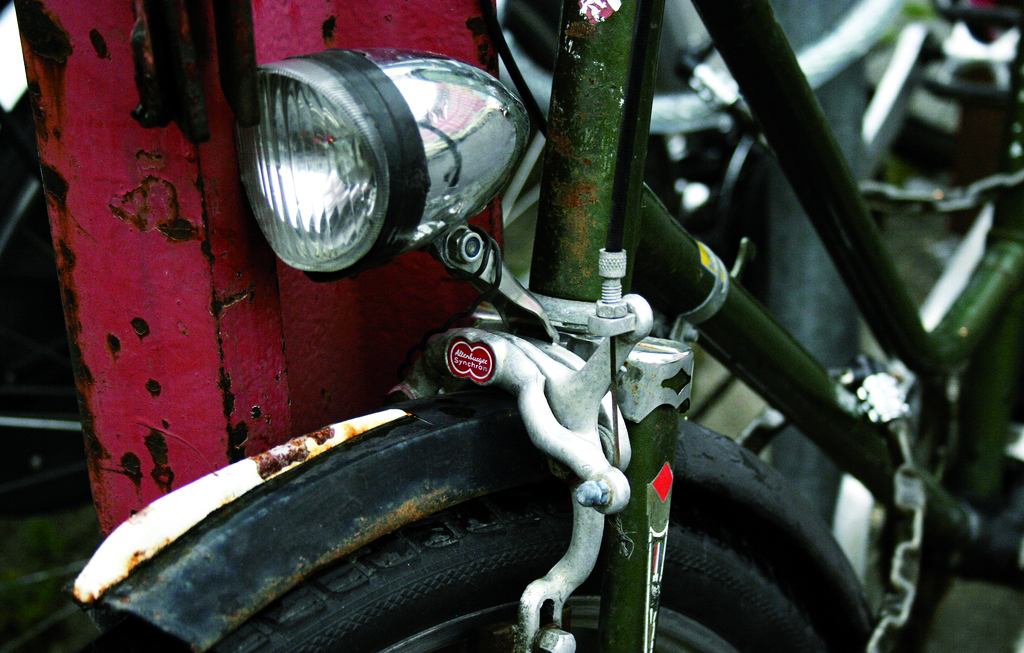
\includegraphics[width={\paperwidth-50mm}]{flickr/725703538_5b9a97ecf2_b}
%	\label{img_bike}
%\end{textblock*}


\section{MVV}
Der Münchner Verkehrsverbund ist der Träger des Großteils des ÖPNV in München.

\subsection*{Mit den öffentlichen Verkehrsmitteln in die Uni}\hfill\\
Die U-Bahnen U3 und U6 halten direkt am Hauptgebäude (Haltestelle Universität).
Die meisten anderen Gebäude sind ebenfalls mit U-Bahn, Bus oder Tram gut zu
erreichen. Genaueres zu den wichtigsten Gebäuden und naheliegenden Haltestellen
finden sich auf der am Ende dieses Heftes zu findenden Karte.

%Informationen zu den anfallenden Kosten für den MVV (Münchner Verkehrsverbund) findest du im Kapitel "`Semesterticket und Ausbildungstarif"'.
%\subsection*{Kosten}\hfill\\
%Für die meisten Studika ist momentan der von der MVV (Münchner Verkehrsverbund) angebotene Ausbildungstarif II am interessantesten. Der Preis richtet sich dabei nach der Zahl der benötigten Zeitkartenringe, die befahren werden. Bevor du dir aber ein Ticket kaufen kannst, musst du dir ein Kundenkarte besorgen. Diese bekommst du im MVG-Kundencenter am Hauptbahnhof, Ostbahnhof oder in der Poccistr.~1--3 (alle zwischen 8:00 und 18:00~Uhr) oder online \newline http://www.mvv-muenchen.de/de/tickets-preise/tickets/schule-ausbildung-und-studium/\newline kundenkarte/index.html\#c9815

%Das Ticket gibt es mit der Gültigkeit einer Woche (9,50 -- 38,90~€) oder eines Monats (34,70 -- 142,00~€) an einem der MVG-Zeitkartenautomaten, in den MVG-Kundencentern oder den MVG-Verkaufsstellen. Monatsfahrkarten gelten bis 12Uhr des ersten Werktags des Folgemonats.\\
%~
%Wenn du in Zukunft günstiger unterwegs sein willst, kannst du bei der Initiative Ausbildungsticket, einem Bündnis aus Studika, Schülern und Azubis mitmachen:\newline \url{ausbildungsticket.de}

%Mehr Infos zum Ausbildungstarif: \url{mvg-mobil.de/tarife/ausbildungstarif.html}
%\chapter{Semesterticket und Ausbildungstarif}

\subsection*{Semesterticket}

\begin{figure}[ht]
	\centering
	\begin{minipage}[b]{0.45\linewidth}
		
\includegraphics[width=\textwidth]{IsarCardSemester-MVG-ICA-Automat}
		%\caption{Isarcard Semester aus einem MVG-Automat}
		\label{fig:isarcardsemestermvg}
	\end{minipage}
	\quad
	\begin{minipage}[b]{0.45\linewidth}
		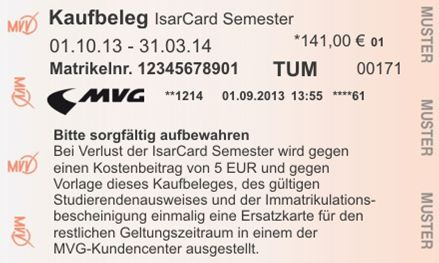
\includegraphics[width=\textwidth]{IsarCardSemester-MVG-ICA-Automat-Kaufbeleg}
		%\caption{Dazugehöriger Zahlungsbeleg}
		\label{fig:isarcardsemesterbelegmvg}
	\end{minipage}
\end{figure}

Dank des \emph{AK Mobilität zum Semesterticket München} \ref{akmobilitaet} hat
München nach vielen Jahren nun auch endlich ein Semesterticket für seine
Studenten. Bei der Zahlung deines Studienbeitrages ist dir sicherlich
aufgefallen, dass du einen Solidarbeitrag in Höhe von 59,00~€ leisten musst.
Diesen Beitrag müssen alle Studika bezahlen - im Gegenzug darf damit das
komplette Netz des MVV befahren werden: täglich von 18--6 Uhr, an Wochenenden
und Feiertagen sogar ganztägig (daher auch ``Partyticket'' genannt).


Möchtest du dein Ticket auch außerhalb dieser Zeiten nutzen, kannst du gegen
eine Zahlung von 146,50~€ an den Automaten der MVG und der
Deutschen Bahn das Semesterticket erwerben. Im Gegensatz zum Solidarbeitrag,
musst du diesen Teil des Tickets aber nicht erwerben, wenn du nicht möchtest
bzw. das Ticket nicht brauchst.

Für die meisten Studika, die den MVV nutzen, dürfte das Semesterticket die
günstige Möglichkeit sein -- es lohnt sich schon, wenn du pro Monat mehr als
24,42~€ in Fahrkarten investieren würdest.

\begin{figure}[ht]
\centering
	\begin{minipage}[b]{0.45\linewidth}
		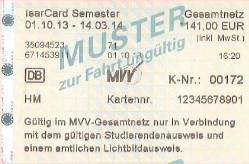
\includegraphics[width=\textwidth]{IsarCardSemester-DB-Automat}
		%\caption{Isarcard Semester aus einem DB-Automat}
		\label{fig:isarcardsemesterdb}
	\end{minipage}
	\quad
	\begin{minipage}[b]{0.45\linewidth}
		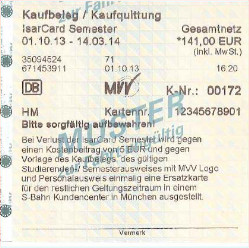
\includegraphics[width=\textwidth]{IsarCardSemester-DB-Automat-Kaufbeleg}
		%\caption{Dazugehöriger Zahlungsbeleg}
		\label{fig:isarcardsemesterbelegdb}
	\end{minipage}
\end{figure}

Das Semesterticket -- sowohl das ``Partyticket'' als auch der Teil mit
Zuzahlung -- sind immer für ein Semester gültig. Hier musst du dich auf die auf
deinem Studienausweis aufgedruckte Laufzeit des Semesters beziehen - die
anderen Hochschulen in München haben teilweise andere Laufzeiten für ihre
Semester. Bitte denke auch daran, dass das Semesterticket immer nur zusammen
mit deinem Studienausweis gilt, welcher wiederrum nur mit einem amtlichen
Ausweisdokument gültig ist.

Wenn du beschließt, ein Semesterticket am Automaten zu kaufen (halte bitte deine
Matrikelnummer zur Eingabe bereit), erhältst du zwei Belege: Ein Mal das Ticket
als solches und einen Zahlungsbeleg. Letzteren solltest du daheim gut aufheben,
denn solltest du dein Ticket verlieren, kannst du einmalig gegen Vorlage des
Zahlungsbeleges und Entrichten von 5,00~€ ein zweites Semesterticket erhalten.

\begin{urlList}
	\httpItem[AK Mobilität zum Semesterticket München]{semesterticket-muenchen.de}{akmobilitaet}
\end{urlList}

\subsection*{Ausbildungstarif}
Für Studika, die nur wenige Monate den MVV in Anspruch nehmen, kann sich unter
Umständen auch der vom MVV angebotene Ausbildungstarif II
\ref{ausbildungstarif} lohnen. Der Preis richtet sich dabei nach der Zahl der
benötigten Zeitkartenringe, die befahren werden. Bevor du dir aber ein Ticket
kaufen kannst, musst du dir eine Kundenkarte besorgen. Diese bekommst du im
MVG-Kundencenter am Hauptbahnhof, Ostbahnhof oder in der \mbox{Poccistr.}~1--3 (alle
zwischen 8:00 und 18:00~Uhr). Alternativ kannst du deine Kundenkarte auch
direkt online \ref{ausbildungstarif-antrag} beantragen und selber Ausdrucken.

Das Ticket gibt es mit der Gültigkeit einer Woche (10,20~€ bis 41,90~€) oder eines Monats (37,40~€ bis 152,90~€) an einem der MVG-Zeitkartenautomaten, in den MVG-Kundencentern oder den MVG-Verkaufsstellen. Monatsfahrkarten gelten bis 12 Uhr des ersten Werktags des Folgemonats.

\begin{urlList}
	\httpItem{mvg-mobil.de/tarife/ausbildungstarif.html}{ausbildungstarif}
	\httpItem{mvg-kundenportal.de}{ausbildungstarif-antrag}
\end{urlList}

\section{Auto}
Du kommst im Allgemeinen mit dem Auto nicht schneller durch die Stadt, als mit dem ÖPNV oder dem Fahrrad. Spätestens bei der Parkplatzsuche vor der Uni wirst du dann merken, dass es bessere Möglichkeiten gibt, in die Uni zu kommen.

	
	\appendix
	
\chapter{Gebäudeübersichten}


\section*{Geschwister-Scholl-Platz 1 (Hauptgebäude)}
\begin{figure}[H]
	\centering
	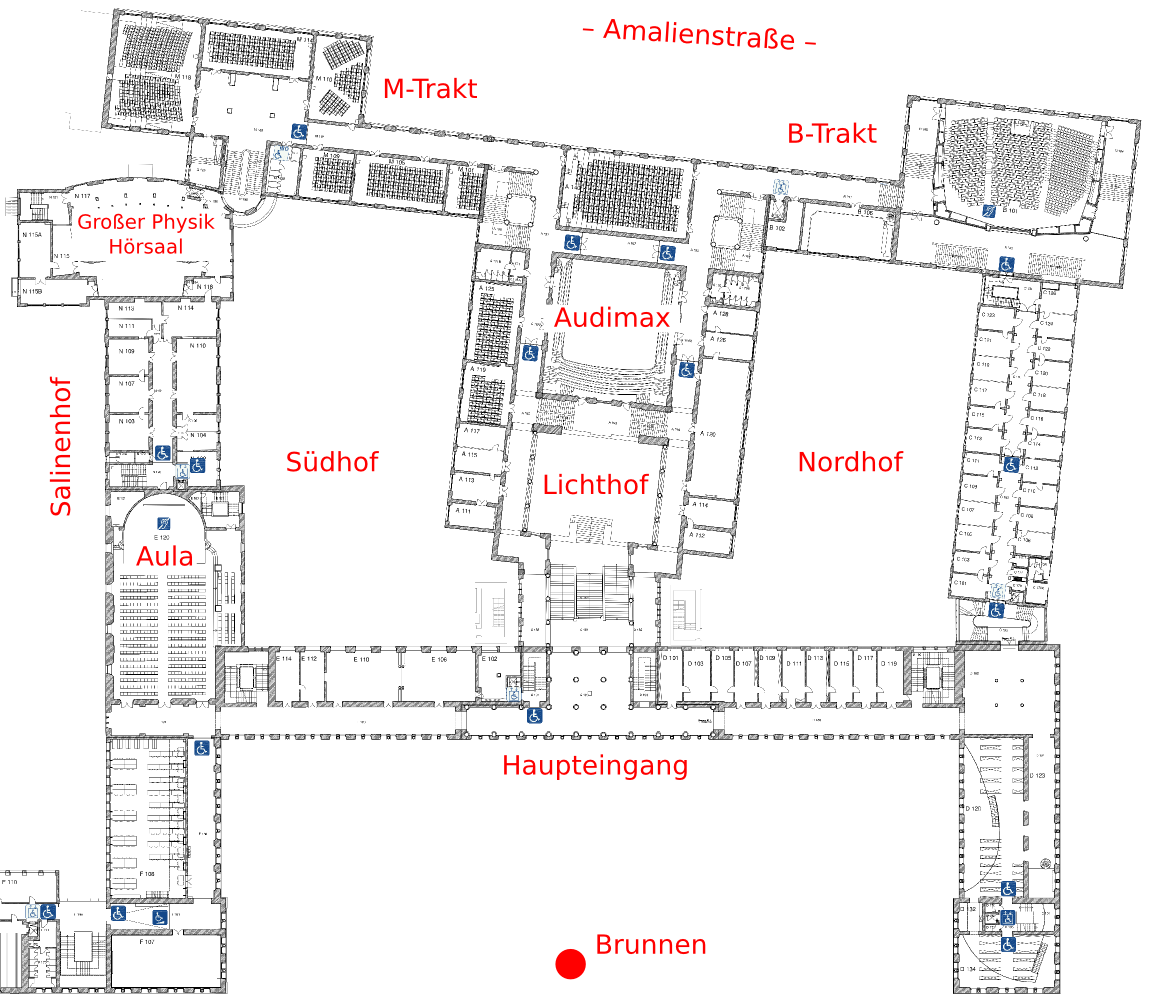
\includegraphics[width=\textwidth]{hauptgeb.png}
	\caption{Erdgeschoss}
\end{figure}

\section*{Theresienstraße 37 -- 41 (Mathebau)}
\begin{figure}[H]
	\centering%
	\begin{minipage}{.5\textwidth}
		\centering
		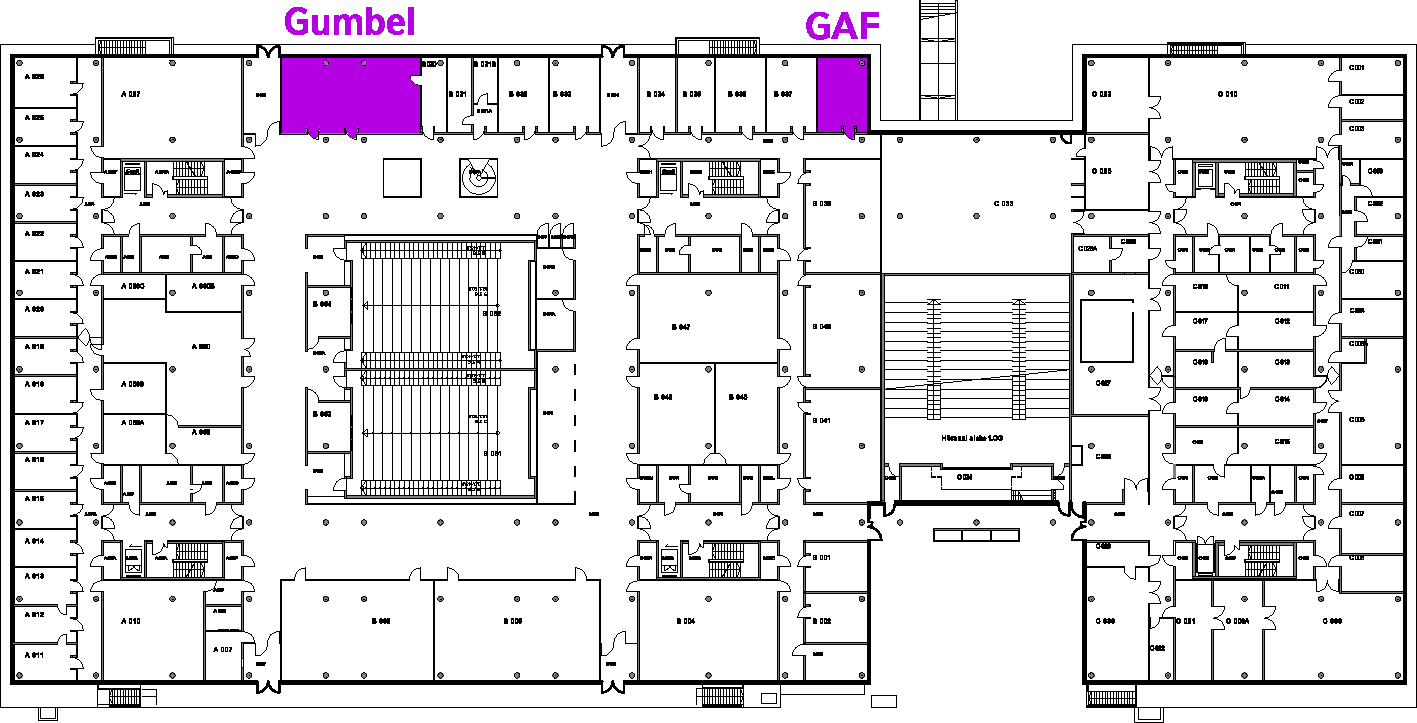
\includegraphics[width=0.65\textheight,angle=270]{mathebau_eg}
		\caption{Erdgeschoss}
	\end{minipage}%
	\begin{minipage}{.5\textwidth}
		\centering
		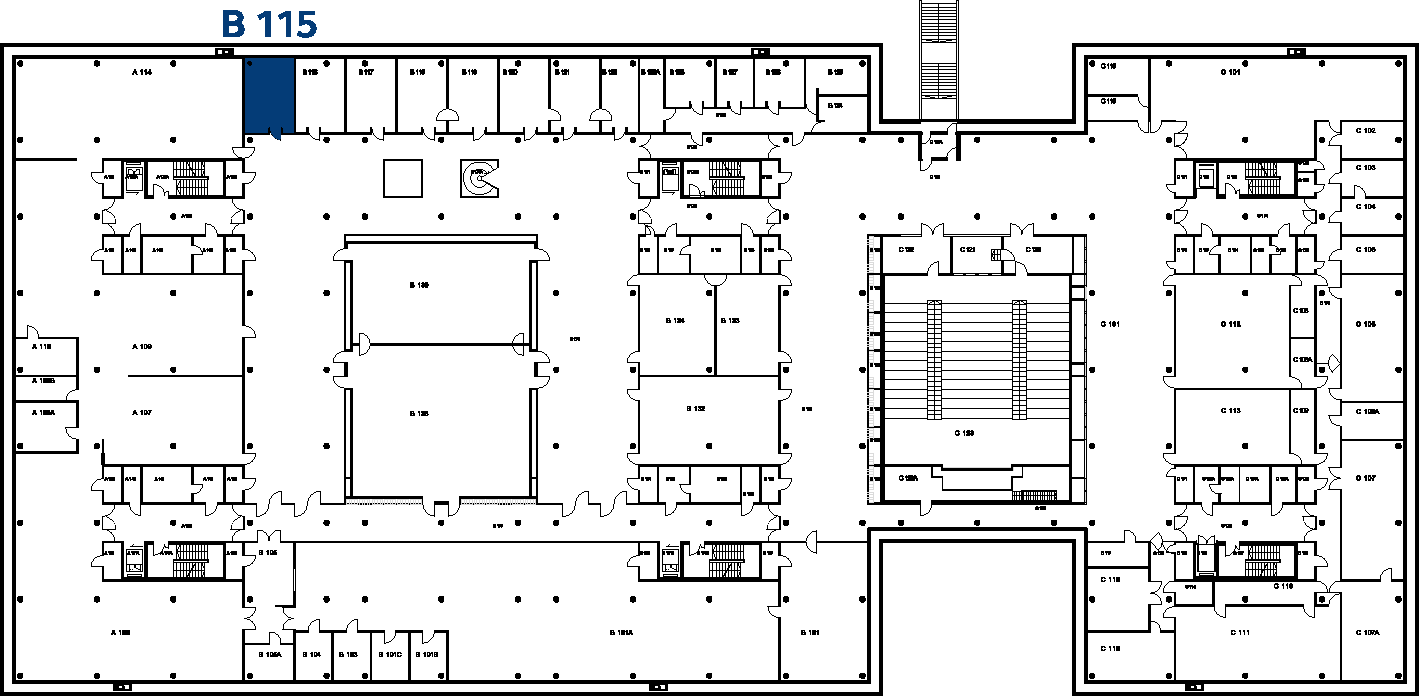
\includegraphics[width=0.65\textheight,angle=270]{mathebau_og}
		\caption{1. Obergeschoss}
	\end{minipage}
\end{figure}

\section*{Oettingenstraße 67\subjectList{\subjectMI{}\subjectI{}}}
\begin{figure}[H]
	\centering%
	\begin{minipage}{.5\textwidth}
		\centering
		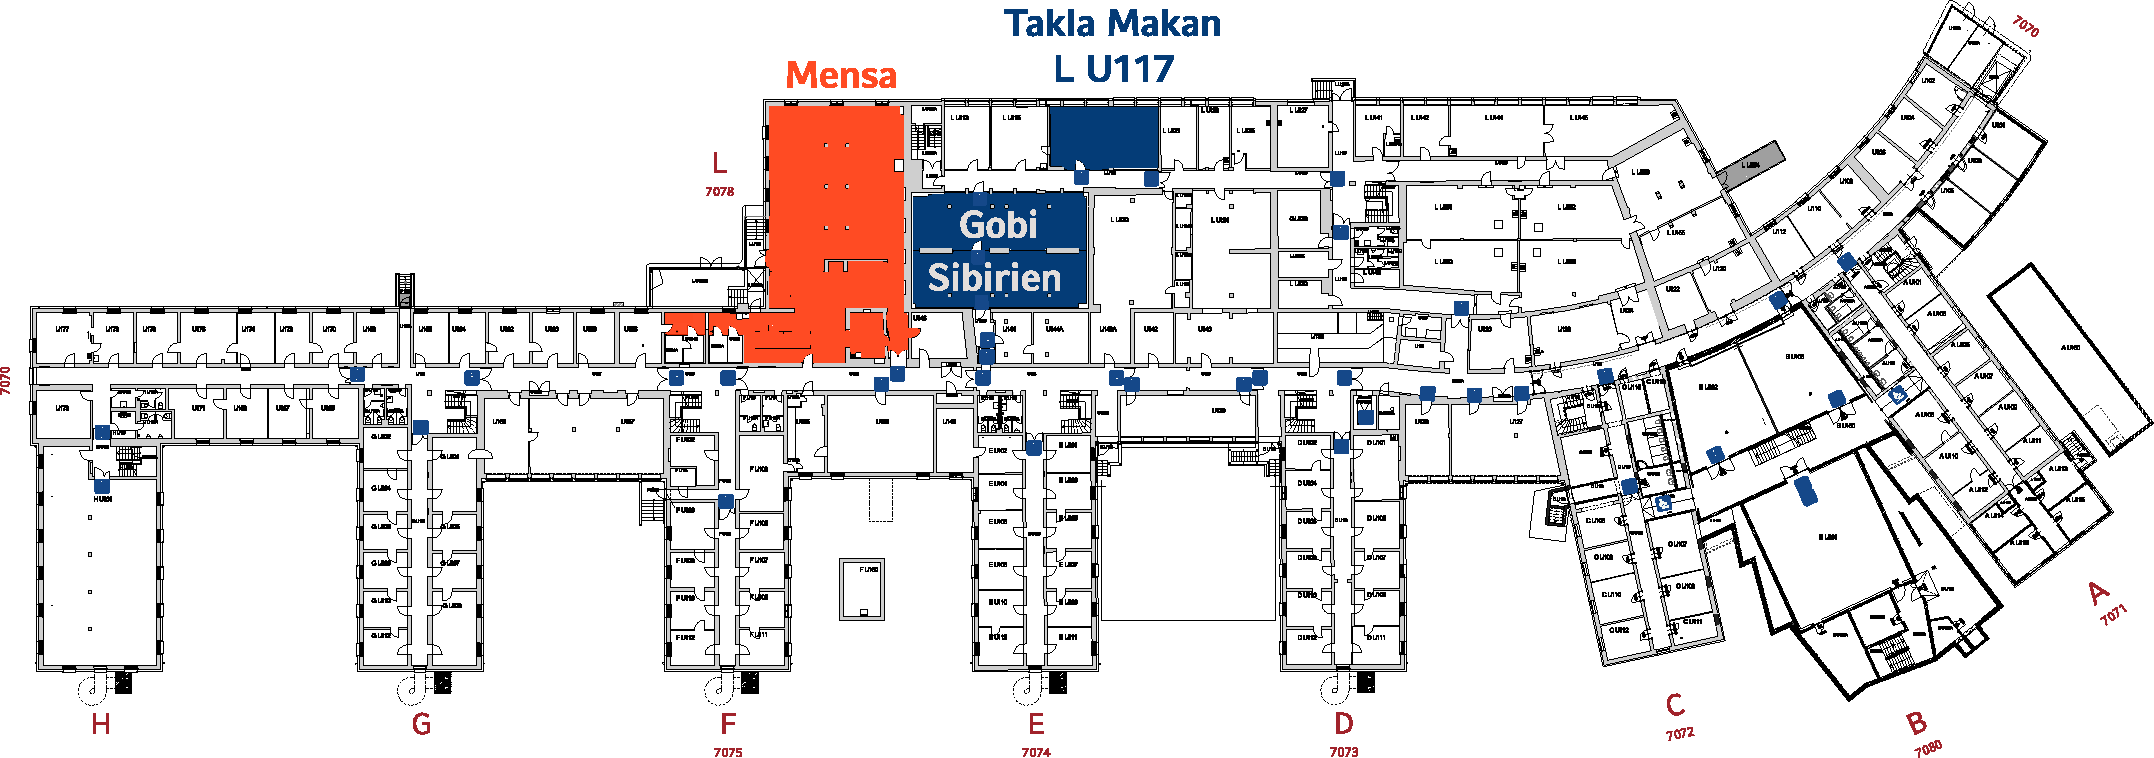
\includegraphics[width=0.85\textheight,angle=270]{oettingen_ug}
		\caption{Keller}
	\end{minipage}%
	\begin{minipage}{.5\textwidth}
		\centering
		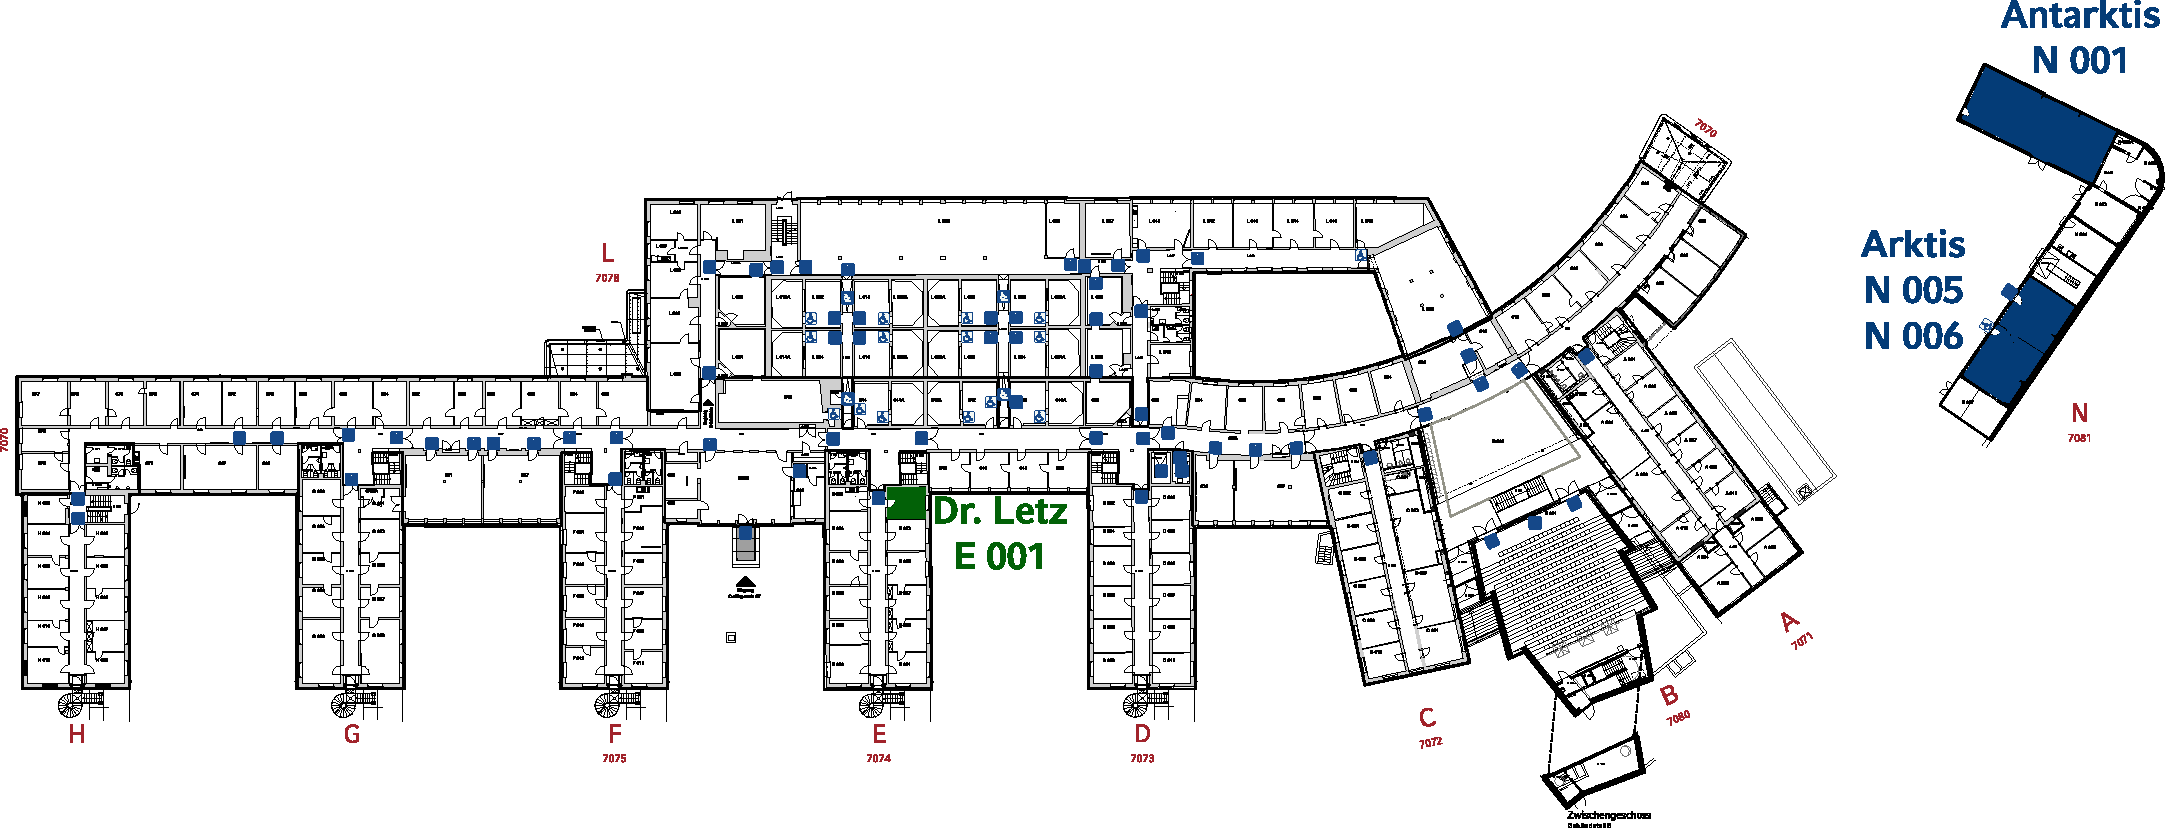
\includegraphics[width=0.85\textheight,angle=270]{oettingen_eg}
		\caption{Erdgeschoss}
	\end{minipage}
\end{figure}

\section*{Schellingstraße 4\subjectList{\subjectP{}}}
\begin{figure}[H]
	\centering
	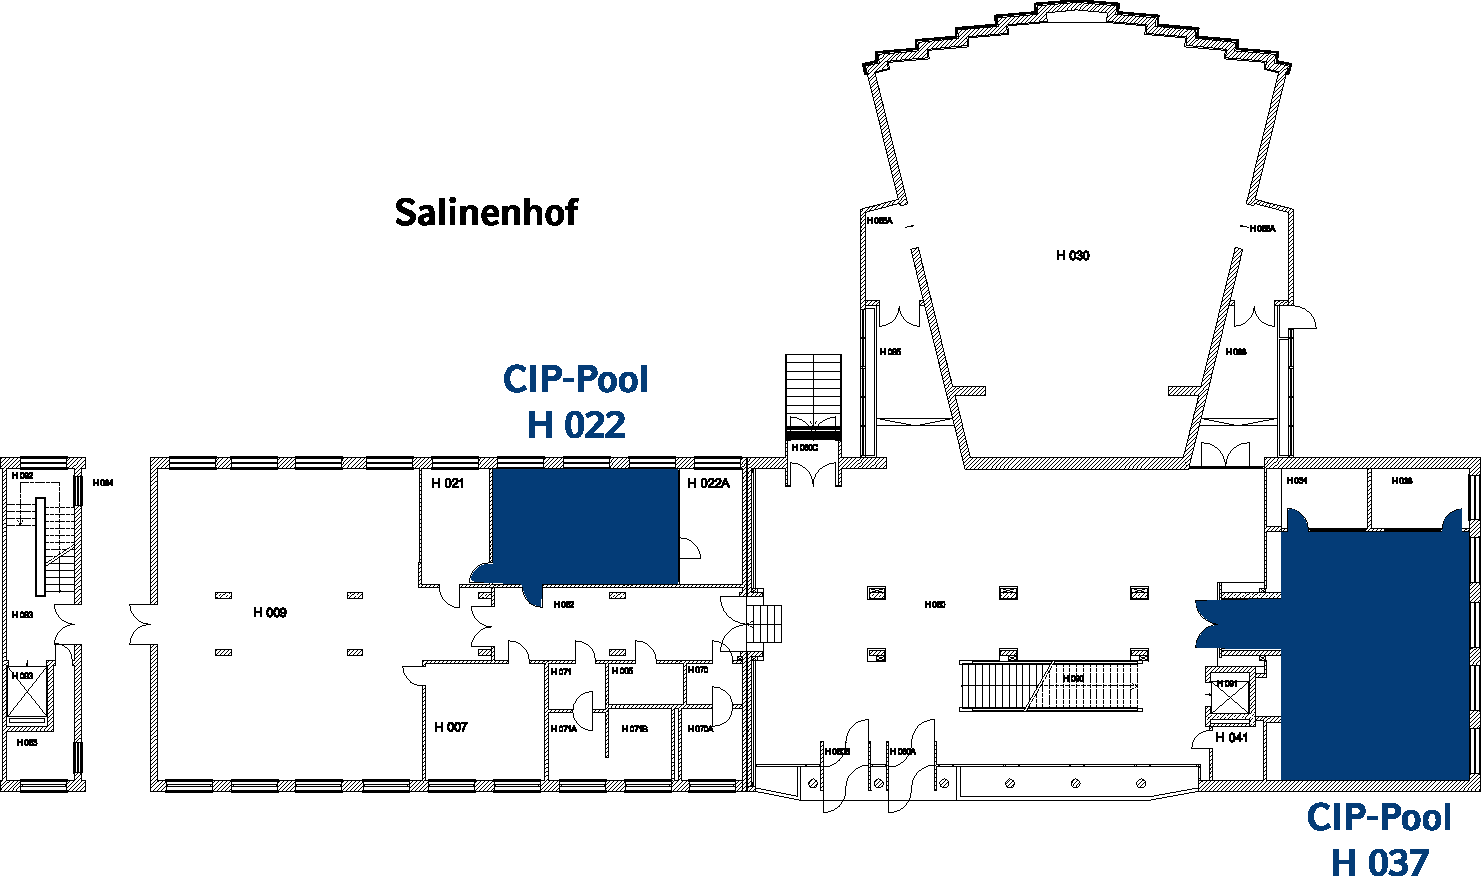
\includegraphics[width=\textwidth]{schelling}
	\caption{Erdgeschoss}
\end{figure}

	\section{Rätselseite}

\textbf{Mini-Sudoku}: Trage in jede Zeile und Spalte
  die Ziffern 1, 2, 3,~4 so ein, dass A~waagrecht, A~senkrecht,
  B~senkrecht und F~senkrecht Primzahlen sind!\\[0.2cm]
\begin{tabular}{ |p{0.8cm}|p{0.8cm}|p{0.8cm}|p{0.8cm}| }
\hline
  a & b & c & d \\[0.8cm]
\hline
  e &   &   &   \\[0.8cm]
\hline
  f &   &   &   \\[0.8cm]
\hline
  g &   &   &   \\[0.8cm]
\hline
\end{tabular}

\medskip
\textbf{Löse folgende Gleichung:}

\[\frac{\textrm{EVE}}{\textrm{D\,I\,D}} = \textrm{0,TALKTALKTALK}\dots\]

Jeder Buchstabe steht für eine andere Ziffer.

\textbf{Visitenkarten:} Welchen Beruf haben diese Personen?\\

\centerline{Hanne Rubbich \textendash{} Ilztal\\[0.2cm]}
\centerline{Richie Hersvogt \textendash{} Zell\\[0.2cm]}
\centerline{Meike Schmettelin \textendash{} Berlin\\[0.2cm]}

\medskip
\textbf{Minesweeper:} Kennst du.  Jedes Level ist eindeutig lösbar.\\[0.2cm]
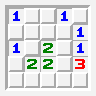
\includegraphics[width=0.45\linewidth]{minepuzzle_gen02tr.png}
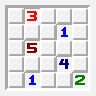
\includegraphics[width=0.45\linewidth]{minepuzzle_gen14tr.png}

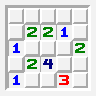
\includegraphics[width=0.45\linewidth]{minepuzzle_gen18tr.png}
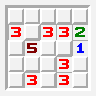
\includegraphics[width=0.45\linewidth]{minepuzzle_gen21tr.png}

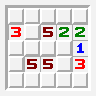
\includegraphics[width=0.45\linewidth]{minepuzzle_gen29tr.png}
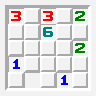
\includegraphics[width=0.45\linewidth]{minepuzzle_gen19tr.png}

\bigskip
\textbf{Kreuzzahlenrätsel:} Jede Summe, und jeder Summand innerhalb der Summe, darf nur einmal auftreten.

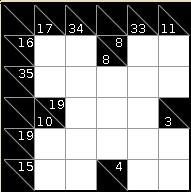
\includegraphics[width=0.9\linewidth]{2011-10-02-134837_191x192_scrot.png}

\end{multicols}


	
\chapter[Abkürzungen]{Häufig gebrauchte Abkürzungen}
\begin{tabular}{l p{10cm}}
BAföG        &Bundesausbildungsförderungsgesetz\\
c.t.        &Lat.: cum tempore (15 min später als angegeben)\\
EWO        &Erstsemesterwochenende\\
GAF        &Gruppe aktiver Fachschaftika\\
g.d.w.    & genau dann wenn\\
LMU        &Ludwig-Maximilians-Universität\\
LPO        &Lehramtsprüfungsordnung\\
LRZ        &Leibniz-Rechenzentrum\\
MVG    &Münchner Verkehrsgesellschaft\\
MVV    &Münchner Verkehrs- und Tarifverbund = \newline MVG + S-Bahn + $\Sigma$ Regionale Busunternehmen\\
N.N.        &Lat.: Nomen nominandus (noch zu nennen)\\
o.B.d.A.    &ohne Beschränkung der Allgemeinheit\\
RBG        &Rechnerbetriebsgruppe\\
RGB             &Rot-Grün-Blau\\
RTFM        &Read The Fucking Manual\\
s.t.        &Lat.: sine tempore (pünktlicher Beginn)\\
StuVe           &Studikavertretung\\
TUM/TU        &Technische Universität München\\
FH/HM        &[Fach-]Hochschule München\\
ZHS        &Zentraler Hochschulsport\\
\end{tabular}




	
	
	\backmatter
	\makeatletter
\@mkboth{\MakeMarkcase{\chaptermarkformat Stundenplan}}%
				{\MakeMarkcase{\chaptermarkformat Stundenplan}}%

\makeatother
%\chapter*{Stundenplan}

\def\timeTableBreak{\\[5.65mm]}
\begin{landscape}
	\centering
	\begin{tabularx}{\columnwidth}{r|X|X|X|X|X|}
	\multicolumn{1}{c}{} & \multicolumn{1}{c}{Montag} & \multicolumn{1}{c}{Dienstag} & \multicolumn{1}{c}{Mittwoch} & \multicolumn{1}{c}{Donnerstag} & \multicolumn{1}{c}{Freitag} \\
	\hline
	08:00 &  &  &  &  & \timeTableBreak\cdashline{2-6}
	      &  &  &  &  & \timeTableBreak\hline
	10:00 &  &  &  &  & \timeTableBreak\cdashline{2-6}
	      &  &  &  &  & \timeTableBreak\hline
	12:00 &  &  &  &  & \timeTableBreak\cdashline{2-6}
	      &  &  &  &  & \timeTableBreak\hline
	14:00 &  &  &  &  & \timeTableBreak\cdashline{2-6}
	      &  &  &  &  & \timeTableBreak\hline
	16:00 &  &  &  &  & \timeTableBreak\cdashline{2-6}
	      &  &  &  &  & \timeTableBreak\hline
	18:00 &  &  &  &  & \timeTableBreak\cdashline{2-6}
	      &  &  &  &  & \timeTableBreak\cline{2-6}
	\end{tabularx}
\end{landscape}

	
	\cleardoubleevenpage
	\begin{fullPage}
		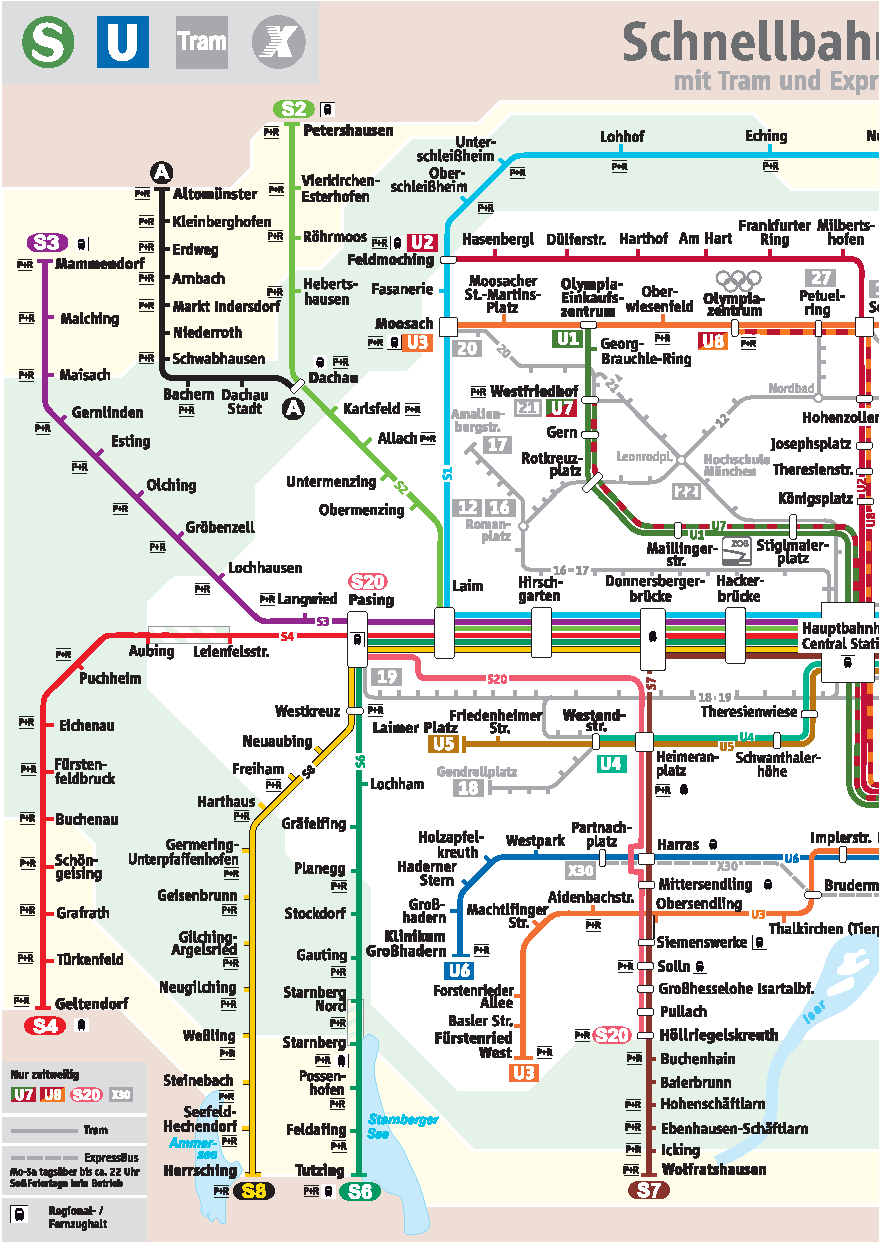
\includegraphics[width=\paperwidth,height=\paperheight]{mvv_links}
	\end{fullPage}
	
	\begin{fullPage}
		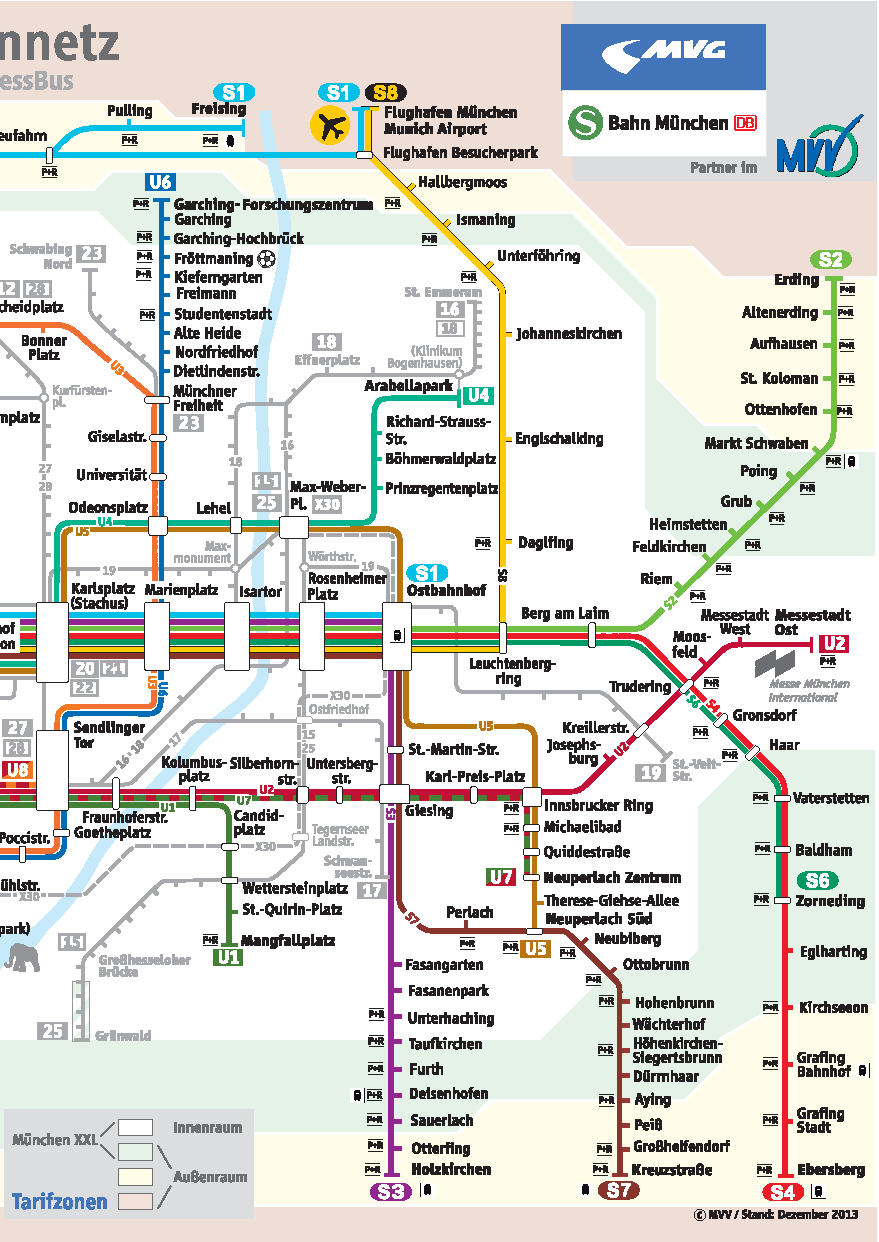
\includegraphics[width=\paperwidth,height=\paperheight]{mvv_rechts}
	\end{fullPage}
	
	\begin{fullPage}
		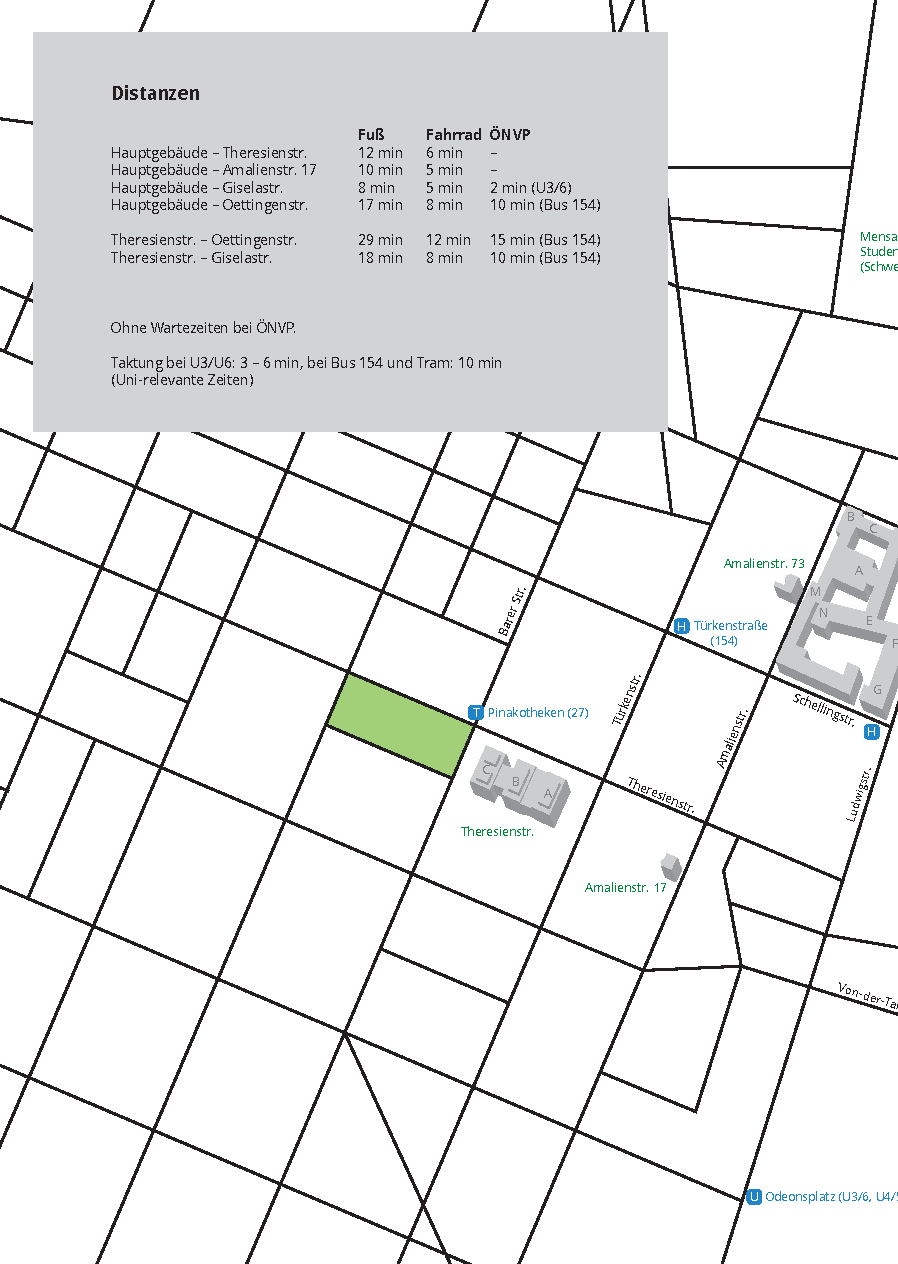
\includegraphics[width=\paperwidth,height=\paperheight]{lageplan_links}
	\end{fullPage}
	
	\begin{fullPage}
		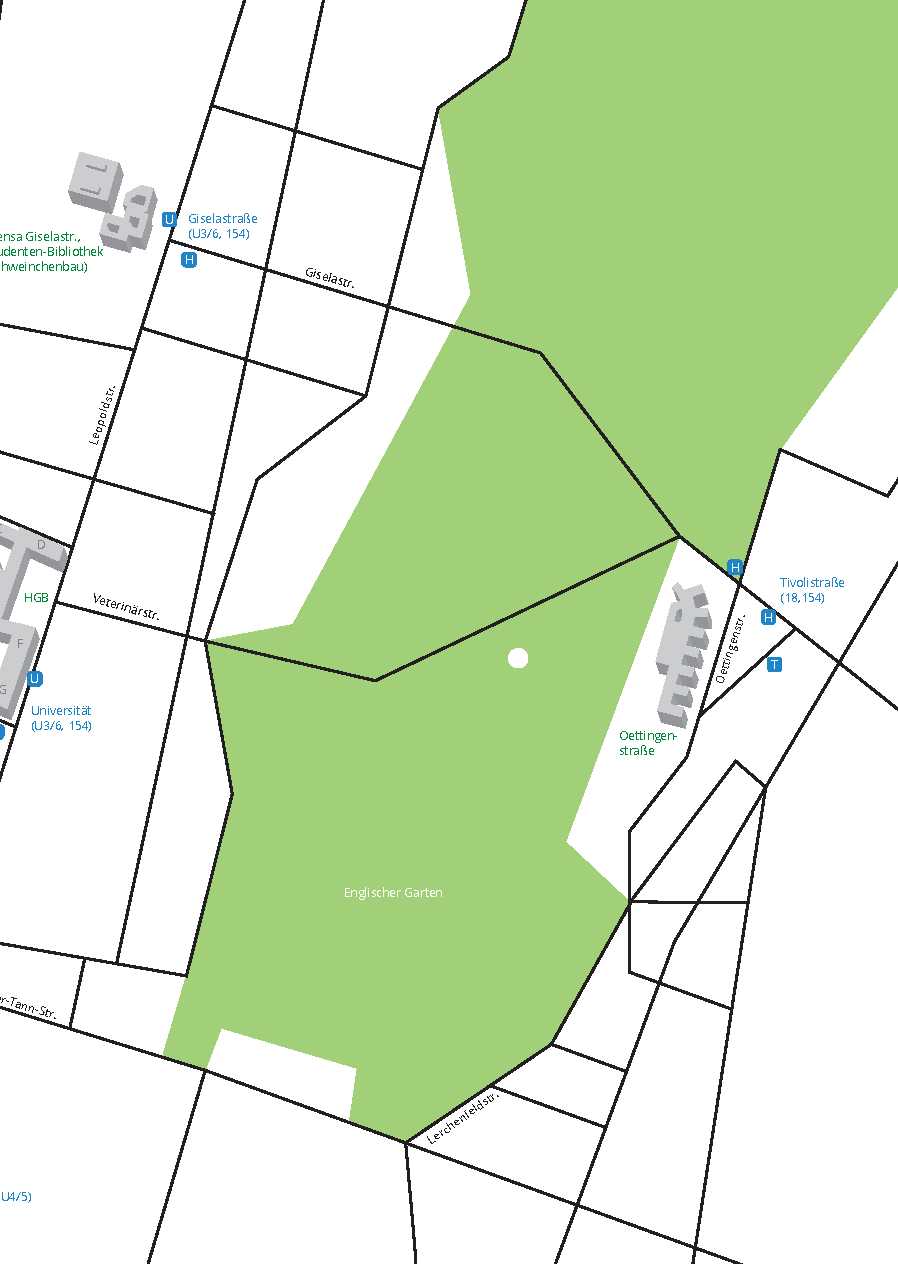
\includegraphics[width=\paperwidth,height=\paperheight]{lageplan_rechts}
	\end{fullPage}
	
	\begin{fullPage}[black]
		
\includegraphics[width=\paperwidth,height=\paperheight]{back}
	\end{fullPage}
\end{document}
